\RequirePackage[l2tabu,orthodox]{nag}

% TODO: decide if one-sided/two-sided
%\documentclass[headsepline,footsepline,footinclude=false,fontsize=11pt,paper=a4,listof=totoc,bibliography=totoc,BCOR=12mm,DIV=12]{scrbook} % two-sided
\documentclass[headsepline,footsepline,footinclude=false,oneside,fontsize=12pt,paper=a4,listof=totoc,bibliography=totoc]{scrbook} % one-sided
\setcounter{secnumdepth}{5}
\setcounter{tocdepth}{5}

% TODO: change citation style in settings
\PassOptionsToPackage{table,svgnames,dvipsnames}{xcolor}

\usepackage[utf8]{inputenc}
\usepackage[T1]{fontenc}
\usepackage[sc]{mathpazo}
\usepackage[american]{babel}
\usepackage[autostyle]{csquotes}
\usepackage[%
  backend=biber,
  url=false,
  style=alphabetic,
  maxnames=4,
  minnames=3,
  maxbibnames=99,
  firstinits,
  uniquename=init]{biblatex} % TODO: adapt citation style

\usepackage{graphicx}
\usepackage{scrhack} % necessary for listings package
\usepackage{listings}
\usepackage{lstautogobble}
\usepackage{tikz}
\usepackage{pgfplots}
\usepackage{pgfplotstable}
\usepackage{booktabs}
\usepackage[final]{microtype}
\usepackage{caption}
\usepackage[hidelinks]{hyperref} % hidelinks removes colored boxes around references and links
\usepackage{float}
\usepackage{dirtytalk}

\addbibresource{bibliography.bib}
\bibliography{bibliography}

\setkomafont{disposition}{\normalfont\bfseries} % use serif font for headings
\linespread{1.05} % adjust line spread for mathpazo font

% Settings for pgfplots
\pgfplotsset{compat=1.9} % TODO: adjust to your installed version
\pgfplotsset{
  % For available color names, see http://www.latextemplates.com/svgnames-colors
  cycle list={CornflowerBlue\\Dandelion\\ForestGreen\\BrickRed\\},
}

% Settings for lstlistings
\lstset{%
  basicstyle=\ttfamily,
  columns=fullflexible,
  autogobble,
  keywordstyle=\bfseries\color{MediumBlue},
  stringstyle=\color{DarkGreen}
}


% TODO: change thesis information
\newcommand*{\getUniversity}{Technische Universität München}
\newcommand*{\getFaculty}{Fakultät für Informatik}
\newcommand*{\getTitle}{Thesis title}
\newcommand*{\getTitleGer}{Titel der Abschlussarbeit}
\newcommand*{\getAuthor}{Aly Saleh}
\newcommand*{\getDoctype}{Master's Thesis in Informatik}
\newcommand*{\getSupervisor}{Prof. Dr.-Ing. Jörg Ott}
\newcommand*{\getAdvisor}{M.Sc. Teemu Kärkkäinen }
\newcommand*{\getSubmissionDate}{Submission date}
\newcommand*{\getSubmissionLocation}{Munich}
\newcommand{\specialcell}[2][c]{\begin{tabular}[#1]{@{}c@{}}#2\end{tabular}}


\textwidth16cm
\textheight22cm

\topmargin0cm
\oddsidemargin0cm
\evensidemargin0cm
\begin{document}

% Set page numbering to avoid "destination with the same identifier has been already used" warning for cover page.
% (see https://en.wikibooks.org/wiki/LaTeX/Hyperlinks#Problems_with_Links_and_Pages).
\pagenumbering{alph}
\begin{titlepage}
  % HACK for two-sided documents: ignore binding correction for cover page.
  % Adapted from Markus Kohm's KOMA-Script titlepage=firstiscover handling.
  % See http://mirrors.ctan.org/macros/latex/contrib/koma-script/scrkernel-title.dtx,
  % \maketitle macro.
  \oddsidemargin=\evensidemargin\relax
  \textwidth=\dimexpr\paperwidth-2\evensidemargin-2in\relax
  \hsize=\textwidth\relax

  \centering

  \IfFileExists{logos/tum.pdf}{%
    
\includegraphics[height=20mm]{logos/tum.pdf}
  }{%
    \vspace*{20mm}
  }

  \vspace{5mm}
  {\huge\MakeUppercase{\getFaculty{}}}\\

  \vspace{5mm}
  {\large\MakeUppercase{\getUniversity{}}}\\

  \vspace{20mm}
  {\Large \getDoctype{}}

  \vspace{15mm}
  {\huge\bfseries \getTitle{}}

  \vspace{15mm}
  {\LARGE \getAuthor{}}

  \IfFileExists{logos/faculty.pdf}{%
    \vspace{20mm}
    
\includegraphics[height=20mm]{logos/faculty.pdf}
  }{}
\end{titlepage}


\frontmatter{}
\begin{titlepage}
  \centering

  \IfFileExists{logos/tum.pdf}{%
    
\includegraphics[height=20mm]{logos/tum.pdf}
  }{%
    \vspace*{20mm}
  }

  \vspace{5mm}
  {\huge\MakeUppercase{\getFaculty{}}}\\

  \vspace{5mm}
  {\large\MakeUppercase{\getUniversity{}}}\\

  \vspace{20mm}
  {\Large \getDoctype{}}

  \vspace{15mm}
  {\huge\bfseries \getTitle{}}

  \vspace{10mm}
  {\huge\bfseries \getTitleGer{}}

  \vspace{15mm}
  \begin{tabular}{l l}
    Author: & \getAuthor{} \\
    Supervisor: & \getSupervisor{} \\
    Advisor: & \getAdvisor{} \\
    Submission Date: & \getSubmissionDate{} \\
  \end{tabular}

  \IfFileExists{logos/faculty.pdf}{%
    \vfill{}
    
\includegraphics[height=20mm]{logos/faculty.pdf}
  }{}
\end{titlepage}

\thispagestyle{empty}
\vspace*{0.8\textheight}
\noindent
I confirm that this \MakeLowercase{\getDoctype{}} is my own work and I have documented all sources and material used.

\vspace{15mm}
\noindent
\getSubmissionLocation{}, \getSubmissionDate{} \hspace{50mm} \getAuthor{}

\cleardoublepage{}

\addcontentsline{toc}{chapter}{Acknowledgments}
\thispagestyle{empty}

\vspace*{20mm}

\begin{center}
	{\usekomafont{section} Acknowledgments}
\end{center}

\vspace{10mm}

\noindent First and foremost, praise be to God through whose mercy all good things are accomplished.\\

\noindent Beyond that, I would like to express my gratitude to my advisor \textbf{M.Sc Teemu Kärkkäinen} for many insightful conversations, useful comments and remarks throughout the master thesis. Furthermore, my sincere thanks and appreciation goes to \textbf{Prof. Dr.-Ing. Jörg Ott} for supervising this thesis.\\


\noindent I thank my wife  \textbf{Hend} for her continuous support, encouragement and motivation in the past two years, she has always been there for me, thank you for never letting me down.\\

\noindent My \textbf{Mom}, \textbf{Dad} and \textbf{Brother}, words are powerless to express my gratitude, I will forever be grateful for everything you have done for me. Thank you for always supporting and encouraging me even though you are in another continent.\\ 






\noindent 


\cleardoublepage{}

\chapter{\abstractname}
In recent years, research and development in Internet of Things, pervasive computing and machine-to-machine communication have been trending  in the computer science field. Thus led to an increase of pervasive use cases aiming to enhance the  life quality of human beings and preserve the environment. In addition to other use cases such as improving the manufacturing  process and providing better health care. Consequently, this has nurtured  the usage of networking concepts such as Information-Centric, Delay-Tolerant architectures and publish-subscribe messaging systems. Despite all that, there is still a lack of frameworks that facilitates the distribution and harmonization of pervasive use cases. A framework that would assist in deploying different use cases to edge devices in a network. %Imagine being able to send a computation to all lamp posts in a specific area that switches them on once they detect a near by motion while taking into account the computation dependencies and required resources. %Further with the same framework but in a another context, being able to shut down all machines in a factory every Friday by a different computation.\\
 Therefore, we propose a software framework for distributing flows which are representations of computations describing use cases to smart devices in a network. The framework also takes care of the flows dependencies, resources, data communication, service discovery, delivering computations and data to challenged networks. It relies on the concepts of pervasive computing, information-centric and delay-tolerant networking. The framework enables the design, distribution, composition, deployment and execution of various flows to carry out different use cases.



\microtypesetup{protrusion=false}
\tableofcontents{}
\microtypesetup{protrusion=true}

\mainmatter{}
\listoffigures{}
\listoftables{}
% !TeX root = ../main.tex
% Add the above to each chapter to make compiling the PDF easier in some editors.

\chapter{Introduction}\label{chapter:introduction}
\section{IoT \& Distributed Sensor Networks}
\subsection{Show how Iot is being currently used, its pros and cons}
\subsection{Give an idea about the devices used to make a distributed sensor network}
\section{Motivation}
\subsection{Show the need to explore Pervasive Computing}

\subsection{Illustrate why it might be better to distribute the data in some cases rather than accumulating it in a single server}

\subsection{Explain why Cloud Computing is not always the right solution in some cases}

\subsection{Explain the need to find IoT devices capabilities and limitations when used for data computation}



% !TeX root = ../main.tex
% Add the above to each chapter to make compiling the PDF easier in some editors.

\chapter{Background \& Related Work}\label{chapter:background}

This chapter describes the concepts and background information that this thesis uses and relies on. It gives a brief introduction about Internet of things and other concepts that emerged from within such as pervasive and fog computing. Moreover, the chapter explains delay tolerant and information centric networking as they play an important role in this thesis. Further, we explain the software platforms and hardware used to implement the system framework.

\section{Internet of Things}

In general terms, IoT refers to a highly dynamic and scalable distributed network of connected devices equipped with context-aware gadgets that enables them to see, hear and think\cite{DAC:DAC2417}. Then, transfer theses senses to a stream of information allowing them to digest the data and act intelligently through actuators if needed. They are also allowed to communicate and share knowledge, which make them smart, powerful and capable of acting independently. Smart devices in an IoT network are heterogeneous in terms of computation capabilities, also each device is energy optimized and able to communicate. Moreover, to qualify for being smart, devices must have a unique global identifier, name, address and can sense the environment. However, the IoT network may also contain devices that are not "smart" which act upon receiving orders triggered through certain circumstances in the network, for example, a lamp post that is set on and off according to network signals. 

Since smart devices have unique identifier and are context-aware, they can be tracked and localized, which is very helpful when performing geospatial computations \cite{Miorandi20121497}. The huge demand on IoT has triggered the development small-scale, high-performance, low-cost computers, in addition, sensors and actuators are getting cheaper, smaller and more powerful which in turn increased the interest even more.
 

The IoT concept can be viewed from different perspectives, it is very elastic and provides a large scale of opportunities in many areas. Currently the number of connected smart devices are estimated in billions, they aim to automate everything around us and are mainly targeted to increase life quality. The broad range of IoT applications include:
\begin{itemize}
\item Smart homes which tend to use sensors and actuators to monitor and optimize home resource consumption and control home devices in a way that increases humans satisfaction. Further, expenses generated from resource usage such as gas, power, water and telecommunications can be sent directly to related authorities without any human intervention \cite{Chan:2008:RSH:1377032.1377113}.  
\item Smart factories also known as "Industry 4.0" the fourth industrial revolution which are optimized machines that communicate together in order to improve the manufacturing process and gather data to analyze factories logistics, pipeline and product availability It also creates intelligent products that can be located and identified at all times in the process \cite{Gilchrist:2016:III:2994178}.

\item Smart cities is one of the most adopted applications in the IoT field, it comprises smart parking, traffic congestion monitoring and control, real time noise analysis, waste management and others.  All this applications need enhanced communication and data infrastructure. It aims to increasing quality of living for individuals\cite{6740844}. 

\item There are also applications in  health care, environmental monitoring, security and surveillance.
\end{itemize}

IoT is very diverse, one way of applying it is to gather data from the smart devices, then process data in the cloud via \textit{Cloud Computing}. Afterwards, results could be sent back to smart devices in order to act somehow. However, exploiting the overwhelming capacity of IoT lead to more specialized and concrete terms that are more focused on pushing computations to the smart devices "Edges" . Consequently, more terms like 
\textit{Edge Computing}, \textit{Pervasive Computing} and \textit{Fog Computing} emerged.


\subsection{Wireless Sensor Networks}
\subsection{Fog Computing}

The fog is an extension to cloud computing at the edge of the network. It provides computation, storage, networking and application services to end-users. Fog and cloud are independent, in fact, cloud can be used to manage the fog. They are also mutually beneficial, some use cases are better deployed in the fog and the other way around. Research yet to determine which applications should go where. The fog is characterized by having lower latency than the cloud, thus are more useful in time critical applications. Also, fog devices have location awareness with a better geographical distribution than the centralized cloud approach. It can distribute the computations and storage between the cloud, itself and idling devices on the network edge \cite{7498684}.

\subsection{Pervasive Computing} 
 Pervasive computing also known as \textit{Ubiquitous Computing} followed from the general IoT networks in which software devices and agents are expected to support and act upon human needs anytime and anywhere without their interference \cite{Chen:2003:OCP:991804.991806}. It is usually integrated with intelligent agents and smart devices which keep learning from human actions and the decisions taken previously to be even more helpful every time. Also, pervasive software agents are context-aware in most of the cases, in which they know what changes are happening around them at a specific point in time and they even hold a history of what has happened in the environment. They also communicate seamlessly in order to share knowledge and help each other take better decisions. Moreover, pervasive devices can be relocated from one place to another, thus changing the network and possibly environment. Therefore, devices can not be addressed with their respective networked addresses because they might eventually change. 

In 1991 Mark Wieser said in the paper describing his vision of ubiquitous computing  \say{The most profound technologies are those that disappear. They weave themselves into the fabric of everyday life until they are indistinguishable from it} \cite{weiser1991ubicomp}. Since then, computing has evolved from using only desktop personal computers to the current phase of wireless sensor networks, small computational devices and distributed systems. Imagine the large scale of applications that could incorporate the computational power, machine learning and context-awareness at the finger tips of  human beings without them even noticing that it exists. In the same paper Wieser also concluded \say{Most important, ubiquitous computers will help overcome the problem of information overload. There is more information available at our fingertips during a walk in the woods than in any computer system, yet people find a walk among trees relaxing and computers frustrating. Machines that fit the human environment, instead of forcing humans to enter theirs, will make using a computer as refreshing as taking a walk in the woods.} 



Figure \ref{fig:pervaisive-computing} shows the architecture of a pervasive environment, in which devices are connected together through a pervasive network which should be lenient to relocating. In addition, each pervasive device has several applications that depend on environment and  context. The pervasive middleware is an abstraction of the core software to the end-user applications.

\begin{figure}[H]
	\centering
	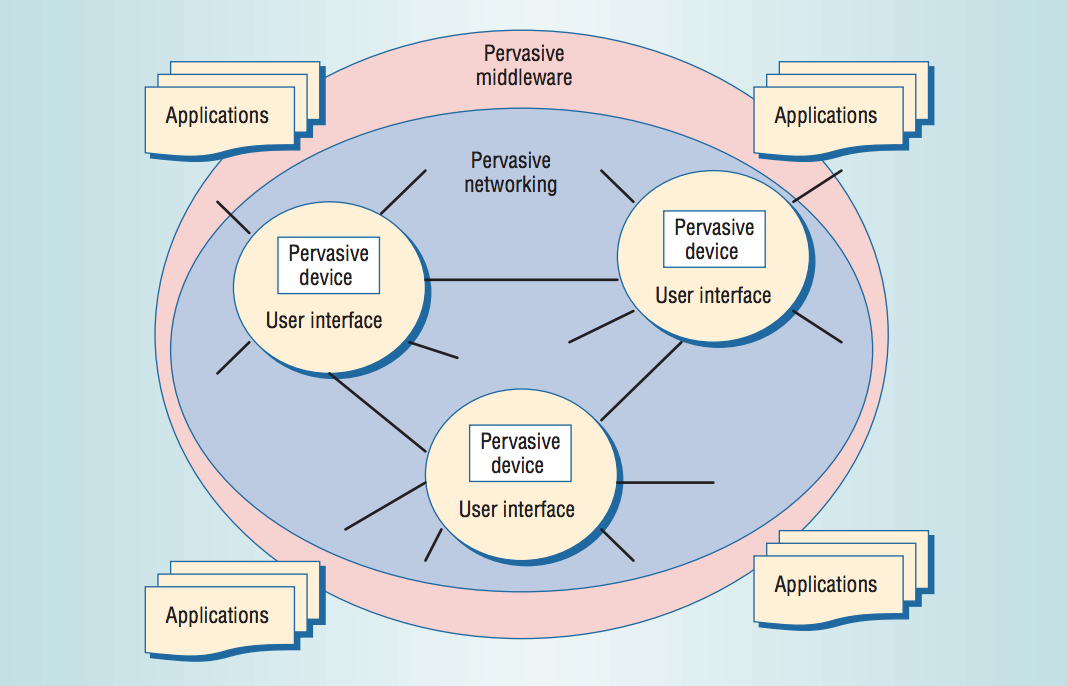
\includegraphics[scale=0.7]{images/pervasive-computing.png}
	\caption{Pervasive Computing environment architecture. \textit{Adapted from \cite{Saha:2003:PCP:642243.642248}}}
 	\label{fig:pervaisive-computing}
\end{figure}

The road to pervasiveness is not paved with gold, there are many challenges that faces the implementation and design of pervasive applications. Some of these challenges are \cite{Schiele2010}:
\begin{enumerate}
\item Devices have become more heterogeneous and the middleware must be able to execute on each of them, therefore, the use of self-contained software environments is advised. For example, using docker as an execution environment for all the heterogeneous devices.
\item Communication reliability is often questioned, in addition,  environments are highly dynamic thus devices are only known at run time.   Therefore, service discovery is a must, either peer-based in which all nodes  take part in the discovery or mediator-bases in which some special devices are promoted to perform service discovery.
\item Sensor availability, readings uncertainty and continuous update of user requirements.
\item Communication and cooperation between devices requires interoperability. There are three different says that allows them to cooperate:

\begin{itemize}
\item Fixed standardized protocol, in which we set some technologies, protocols and data formats in order to be used across the system.
\item Dynamically negotiated, in which devices are allowed to negotiate on which protocols and data formats to use  at run time.
\item Using interaction bridges that map between different approaches and protocols.
\end{itemize}

\end{enumerate} 








\section{Networking}
\subsection{Information Centric Networking}
Information Centric Networking (ICN) is a concept that focuses on content sharing and distribution. In contrast to current network approaches which are host-centric where communication takes place between hosts such as servers, personal computers, etc. ICN was brought to light as a result of the increasing demand on content sharing in highly scalable, distributed and efficient fashion. ICN compromises network caching, replication across entities and resilience to failure.

The content types includes web-pages, videos, images, documents, streaming and others which are titled Named Data Objects (NDO). The NDO is only concerned by its name and data. As long as name identity is preserved, it does not matter where the NDO is going to be persisted, what is the storage method or which type of transport procedure is used. Therefore, copies of NDO are equivalent and can be supplied from any location or replica across an ICN network. However, since the name represents its identity, ICN requires unique naming for individual NDOs.

ICN also provides an Application Programming interface (API) that is responsible for sending and receiving NDOs. The two main roles in this API are the producer who produces content to a specific name and the consumer who asks if an NDO is available by its name. There is also the publish-subscribe approach in which a consumer registers for a subscription to a certain name and gets notified whenever new content is available. This caters for  decoupling between producers and consumers. 

However to ensure that an NDO goes from one entity to another, a consumer request must go through two different routing phases. The first is to find a node that holds a copy of the  NDO
and deliver the request to that node. The second is to find a routing path back from the receiving node to requester carrying the required NDO. This can be achieved in two different ways: i) \textit{name-resolution} in which a resolution service is queried in order to find a way to locate a source node, ii) \textit{name-based routing} in which the request is forwarded to	 another entity on the network based routing algorithms, policies and cached information.

ICN caches are available on all nodes, requests to an NDO can be served from any node having a copy in the cache. An NDO can be cached on-path from sender to receiver or off-path through routing protocols or by registering it into a name-resolution service\cite{6231276}.


\subsubsection{Content Centric Networking}

Content centric networking (CCN) is an architecture based on the ICN concept. Namespace in CCN  is hierarchal, for instance, \verb|/tum.de/connected-mobility/iot| matches the figure \ref{fig:ccn-namespace}. Names do not have to be meaningful or readable, they can include hashes, timestamps, ids, etc. A request matches an NDO if its name is a prefix of any named object, for example,  a request with the name  \verb|/tum.de/connected-mobility/iot| matches an NDO with the name  \verb|/tum.de/connected-mobility/iot/pervasive-computing|.\\ CCN natively support on-path caching, however, off-path can also be supported\cite{6563278}.
\begin{figure}[H]
	\centering
	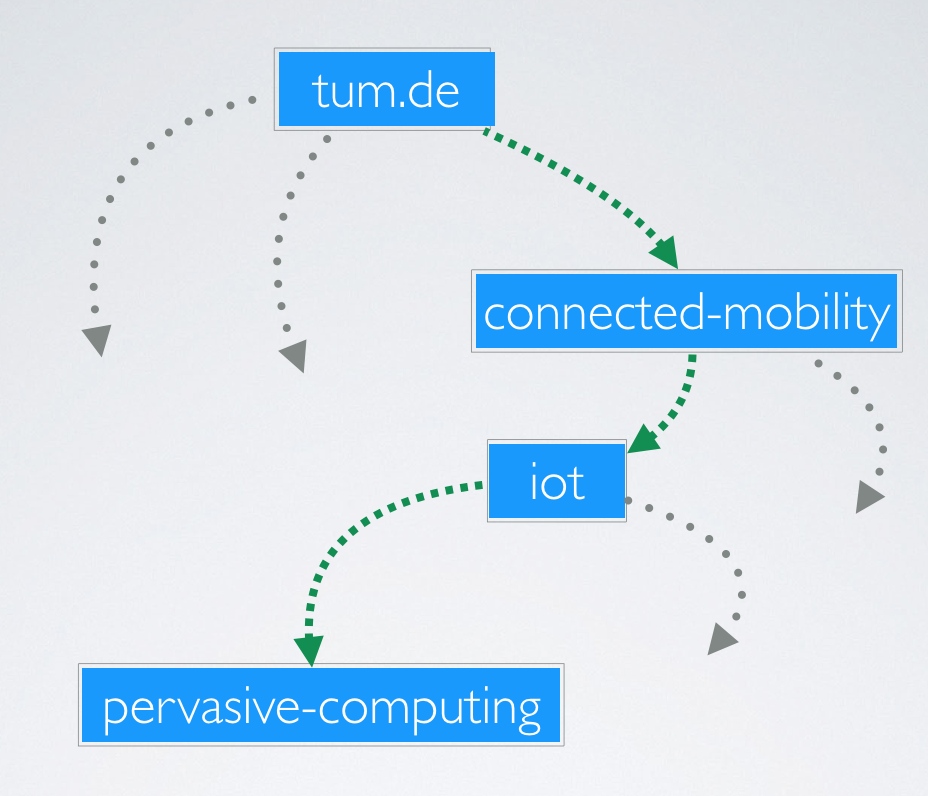
\includegraphics[scale=0.3]{images/namespace.png}
	\caption{Hierarchal namespace example for CCN}
	\label{fig:ccn-namespace}
\end{figure}

Each node in the network contains a \textit{Content Router} which includes three data structures \cite{6563278}\cite{6231276}. 
\begin{itemize}
\item Pending Interest Table (PIT) which stores the subscriptions and interests of NDOs. The subscription does have to originate  from the node itself, rather can be a forwarded from another node. Once an interest reaches a content source and the data is retrieved, the PIT entries serves as a trail to the original subscriber and is removed afterwards.

\item Forwarding Information base (FIB)  stores a mapping that indicates which node should the request be forwarded to. The FIB uses longest common prefix in order to determine the next hop. Multiple entries are allowed and can be queried in parallel.
\item Content Store (CS) which is basically the cache that stores the NDOs and uses \textit{least recently used} (LRU) eviction strategy. Caches with high hierarchy posses a larger storage to be able to store popular NDOs which might get evicted due to  lower storage down in the hierarchy
\end{itemize}  

\begin{figure}[H]
	\centering
	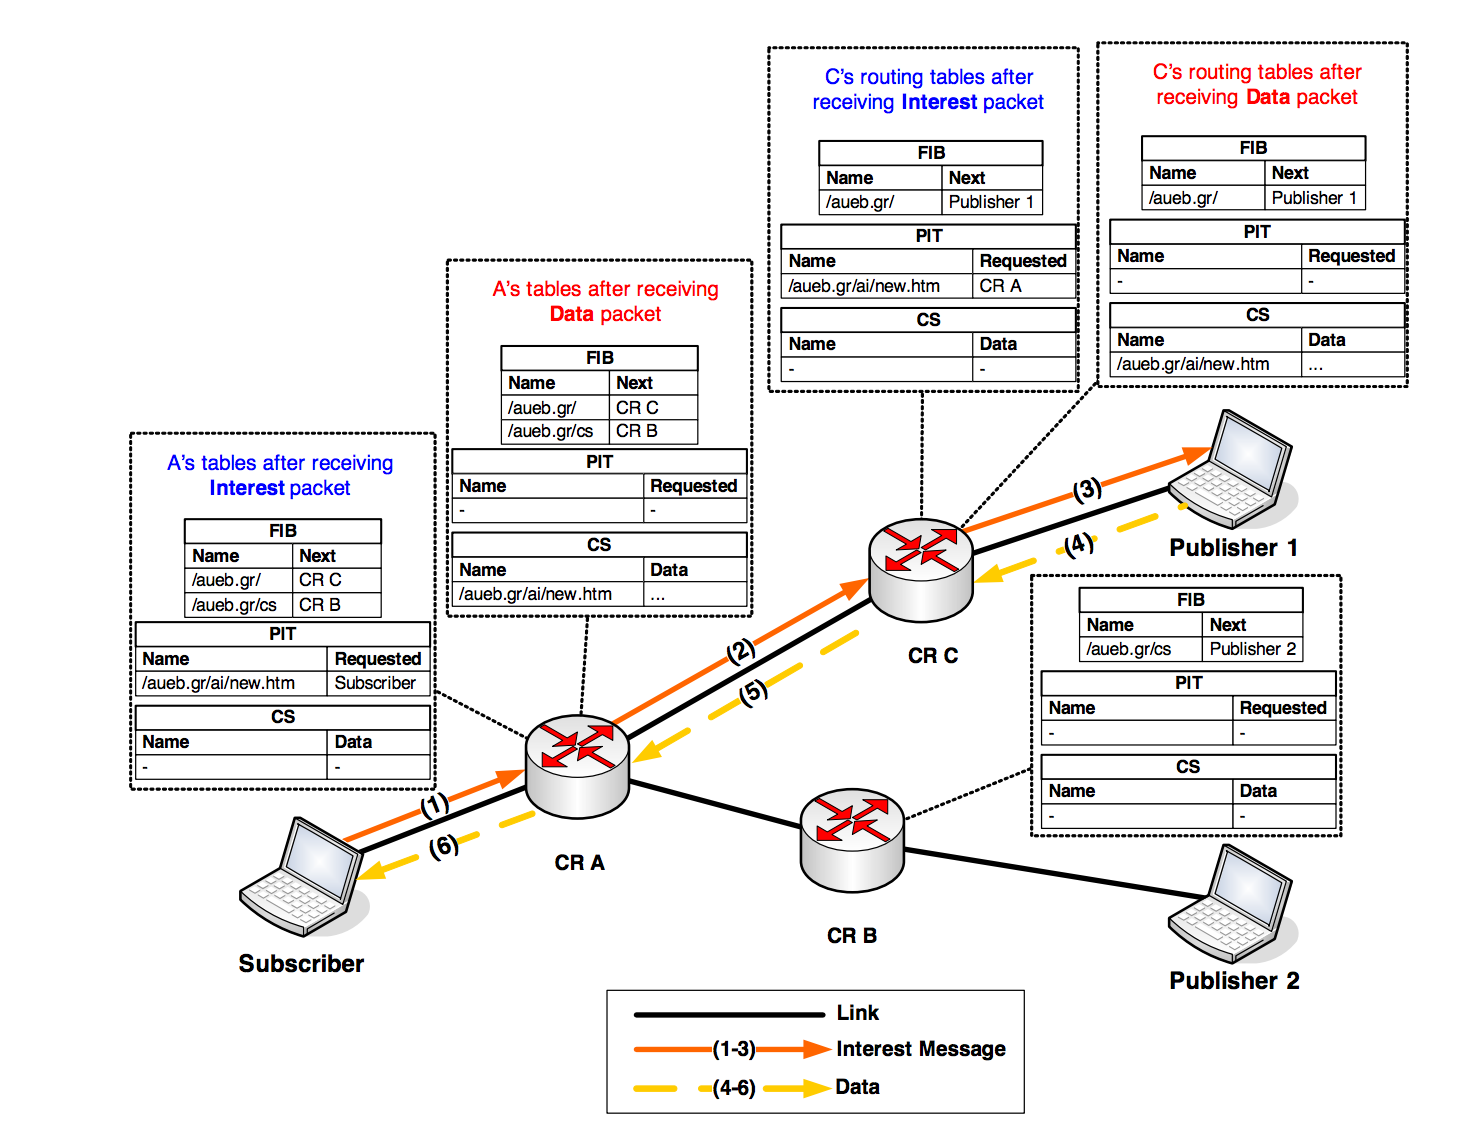
\includegraphics[scale=0.55]{images/ccn2.png}
	\caption{Content centric networking architecture and flow \textit{Adapted from \cite{6563278}}}
	\label{fig:ccn}
\end{figure}

Figure \ref{fig:ccn} describes the flow and state of PIT, FIB and CS of network nodes when receiving the interest message and after acquiring the data. Notice that all the PIT entries have been erased after acquiring the data and CSs have been updated.


\subsection{Delay Tolerant Networking}


\section{Used Platforms}
\subsection{Node-Red}
\subsection{SCAMPI}
\subsection{Raspberry Pi}
\subsection{Time-series Databases}

%\section{Illustrate what are the ideas and possible network mechanisms and protocols that could be used data transfer}
%\subsection{Server To Server }
%\subsection{Server To Device }
%\subsection{Device To Device }



\chapter{Framework in Theory}\label{chapter:Foundation}
In this chapter we explain the framework model in theory, the key concepts behind it, challenges facing the design and their possible solutions.


\section{Foundation}
	The fundamental core element of this framework is the computational unit, which is responsible for describing the use case. One possible abstraction of the computational unit is the \textit{flow}, which is a purposeful unit of computation that contains sequentially meaningful instructions. Also, it can be either standalone self-contained computation or interactive in which they collaborate with other flows for data gathering, sharing and processing. Moreover, the flow is composed of elements which could have a significant meaning such as snapping a photo or could act as an intermediary to harmonize data as shown in figure \ref{fig:flow}. 
	
\begin{figure}[H]
	\centering
	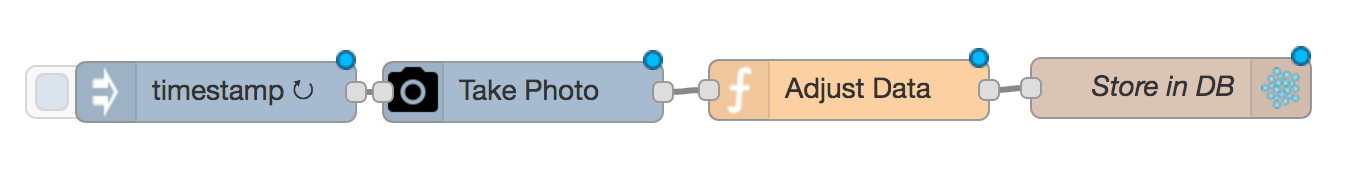
\includegraphics[scale=0.5]{images/db-out.png} 
	\caption{A node-red flow that stores an image in a database every time interval}
	\label{fig:flow}
\end{figure}

After having defined flows, it is important to give an idea on how they end up being executed. To begin with, we must address the challenge that flows are distributed in the sense that each flow could reside on different node. In addition, as previously mentioned, flows may be interactive, therefore, they need a way to communicate through distributed systems. Moreover, since nodes might be disconnected,  the communication mechanism must guarantee that there  exit  a way  in which data could be transfered between these disconnected nodes. Furthermore, it  should handle sending the computations themselves from one node to another, at the end we would like to be pervasive and manage sending computations everywhere.

 Another challenge that faces the flows execution, is the dependencies and resources which could be demanded in order to carry on the execution. They vary from one use case to another, thus needs to be orchestrated across nodes through messaging system.

Now assuming that we can send flows to the nodes, make them communicate and care for their dependencies and resources, one aspect remains, which is triggering the execution of flows. There are multiple ways to start carrying on an execution, one simple example is a time interval trigger as shown in \ref{fig:flow}. Other ways include, starting computation execution when new incoming data has been received or other events have been triggered.\\




 A flow should be modular having a specific functionality with defined interfaces that helps in reducing the complexity, allowing re-use and re-assembly. Moreover, since flows need to interact and exchange data, they should be composable. Think of composability as LEGO parts that need to be assembled in their correct positions in order to create a figure, however in contrast to individual LEGO parts which do not have a meaning on their own, individual flow elements could serve a specific purpose besides their global one. To establish flow composability in our context, we need to be able to match the output data of one flow to the input data of another, no matter whether the flows are on the same node or distributed, connected or disconnected. For instance in general terms, if we have a flow \(f_1\) that takes \(A\) as input and gives \(B\) as an output
\[ f_1 : A  \to B  \]
then we have another flow \(f_2\) that takes \(B\) as an input and gives a new output \(C\)
% the output of \(f_1\) and produce a new result and so on. 
\[ f_2 : B  \to C  \]
we should be able to compose a new flow taking \(f_1\)'s input and giving \(f_2\)'s output, resulting in flow \(f_3\) which is a composite of both.
\[f_3: A \to C = f_2 \circ f_1\]
Since composability should also be valid in a local or distributed environment. Thus, in the first case of local flow composability, there should be a way to connect the output of a flow to the input of another as shown in \ref{fig:compose}. On the other hand if it is distributed composability, the messaging system should connect the dots and serve as a broker to deliver the data.

\[a \in A, \, b \in B, \, c \in C\]
\begin{figure}[H]
	\centering
	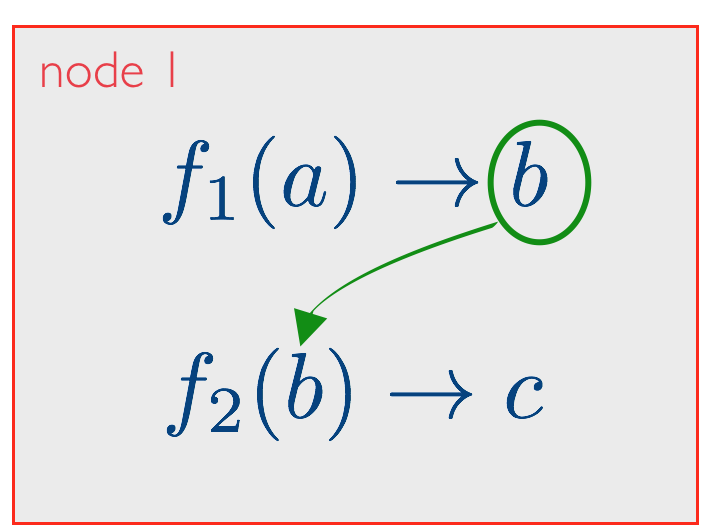
\includegraphics[scale=0.3]{images/local-compose.png} 
 	\caption{A node containing two composable flows}
	\label{fig:compose}
\end{figure}
\begin{figure}[H]
	\centering
	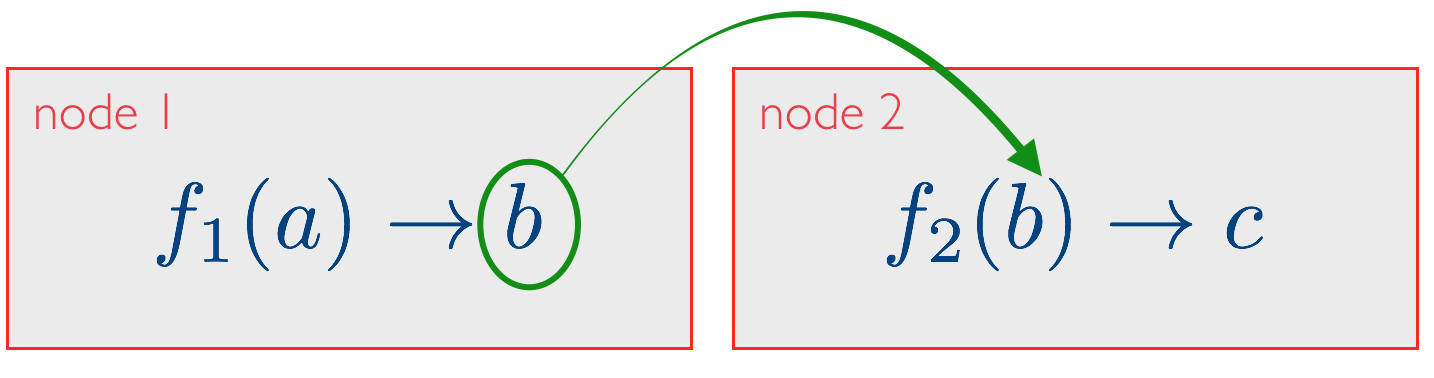
\includegraphics[scale=0.4]{images/distributed-compose.png}
	\caption{Two separate nodes having distributed composability}
	\label{fig:compose2}
\end{figure}


\section{Computational Model}

Below we present the computational model as an abstraction for the framework design, it explains the components, challenges and the possible solutions that could be implemented to overcome these challenges. 	

\subsection{Distributed Nodes \& Flows}
In order to start with the framework explanation we must understand the idea behind pervasiveness. Pervasive computing relies on the idea of pushing flows to the edges "nodes" and thus it is fundamentally distributed. A system is distributed if its components  are on networked computers which communicate only by sending and receiving of messages \cite{DSYS} which is exactly the case. Now in our model, each node should be capable of executing flows and producing results as long as it  has the required dependencies and resources. Moreover, to ensure that flows are composable, nodes should be able to communicate seamlessly even though nodes hosting this flows might be disconnected.



Turning to flows, in essence every challenge related to making the nodes distributed also apply to flows because nodes host flows. However, there are more to flows, distributing them across nodes could have different semantics and approaches depending on the use case.
 Lets us first consider the two different semantics, a flow could be sent on random basis to the nodes, and at the contrary, it could also be sent to specific nodes. This provides flexibility in applying the use case without wasting resources, in addition, it magnifies the effect of locational context in case we want to send a computation to a specific place.
 Moving on to approaches, a flow could be distributed across the nodes in a multiple ways explained as follows: (i) flows are pushed to all the available nodes even if they are disconnected (ii) flows are sent to \textit{n} number of nodes whether they are selected or picked at random, (iii) choosing only one node to execute a specific flow. As a result, the communication model is one of the most crucial parts to guarantee a distributed system, it should have the flexibility to provide these approaches and overcome the hurdle of disconnected nodes.
 

Another main challenge is to actually find the connected nodes. Distributed and pervasive environments are dynamic, their components are not known to be live or dead at compile-time. Thus the framework should be able to run service discovery at run-time in order to find the connected nodes or it should be able to broadcast its message to all the other nodes and receive them as well. Otherwise, the approach would not qualify to be a distributed system. 






\newpage


\subsection{Dependencies}

Dependencies are one of the main requirements of computation execution, dropping one or more dependency would definitely stop the execution from proceeding. Thus, we need to deal with them and make sure they do not introduce any impediments during execution.  There are two types of dependencies; the static software frameworks that the whole design relies on and must exist on each node, and the dynamic dependencies that are specific to each computation.

First, are the static dependencies are mainly the common libraries and software that most of the computations would require, they represent the base of framework. That is why these dependencies are installed to each node in our design, examples of these dependencies include the operating system, data store and any other standard or custom libraries that are mandatory for the computation to run. In addition to, the messaging system which implements the communication model allowing interaction between nodes. 

 Second, are the dynamic dependencies which are specific to each computation such as additional scripts, configuration files or libraries. In this case, they cannot be installed at node initialization since we can not know what are the custom dependencies any computation would need beforehand. Therefore, the computational model design should allow a way to configure additional dependencies. Moreover, the communication mechanism should support this configuration and grant a way to carry the configured dependencies forward to other nodes.
 
 
  Dynamic dependencies creates a bit of ambiguity, suppose that the dependency which is being sent by means of the communication mechanism is already on the receiving node. This introduces a  versioning problem, also what makes it more complicated, is that the node does not know if it possesses an older version of the dependency or a newer one. Furthermore,  imagine there is a computation on the node that uses an older version of the same library while the maintainer is sending a new computation with a newer version of the same library that is not backward compatible. 
  
   Nevertheless, there are multiple possible solutions to remove the ambiguity and make the custom dependency shipping more concrete; one solution would be to give the dependencies different names according to their versions before shipping them, hence, any different version would not replace the existing ones. Another solution would be to design a system that links each running computation on the node to its dependencies and once a collision appears, the new computation renames its dependency and uses the renamed one.
 

\subsection {Resources}


Resources are a different type of dependency which are also necessary for computations to run. However, they might differ or not exist at all on each node. If one of the needed resources is missing then the computation could be either dismissed or queued depending on the type of resource. Moreover, the maintainers cannot make any assumptions about the resources, meaning, an assumption stating that each node has a camera is not necessarily true. Since the resources cannot be standardized across all nodes, each computation must provide meta data expressing the resources it is going to require, also, the node must realize its available resources. Then a node can check against its capabilities and decide whether it could carry out the execution or not. There are two types of resources; sensors and actuators which are used throughout a computation, and the hardware resources which influences the performance requirements of a specific computation.


\subsubsection{Sensors and Actuators}

  Sensors and actuators are resources attached to a node such as cameras, temperature and gas sensors. Executing a computation missing this type of resource on a node should have a lower possibility of being queued, since its highly unlikely that this hardware resource would be attached soon. A node should be aware of its available resources, otherwise, it would not be able to compare the requirements of incoming computations against its capabilities. Hence one possible solution, is for each node to have a specification file as a static dependency stating its available resources.
  
  However sensors and actuators are dynamic, they can be added or removed on demand, therefore, having them in a specification file as a static dependency which is only set at initialization time will be troublesome. Of course, we can always edit the specification file once we change the state of any of these resources, but this solution is not very efficient nor scalable, as it increases the manual work. It would be much easier if the node could run resource discovery to find its attached resources each time it receives a computation.
  
  Moving on to consider computations acquiring the same resource at the same time, for instance, two computations that want to take a photo at the same time. This is problematic because whichever computation acquires a lock on the camera first will succeed while the other will fail. Therefore as a resolution, we could use resource decoupling; instead of having the computation ask a specific resource directly for information, the  data will be pushed into a database. Afterwards, the different computations could query the data from a database.
  
  

\subsubsection{Hardware Resources }

The second type of resources is related to the node performance, its power and memory capabilities, it is heavily biased by the processor of the node and its random access memory type and size. Computations vary in terms of resource consumption and hence a heavy computation should not be deployed to a node which is already loaded. 

Considering that each computation model has meta-data describing its resource consumption, then it is possible to decide if it is going to be deployed on a specific node or not. Additionally, if it is not going to be deployed then it should be decided whether the computation is going to be queued or dismissed according to the possibility of acquiring the resource.

The idea of queuing computations however develops a scheduling problem. Since we have a queue of computations inside each node, we will have a race condition on which computation should be deployed first according to available resources. Furthermore, since some computations might be dismissed, a rather bigger scheduling problem will come up when we try to fit the all computations across nodes in the whole system framework 
\newpage




\subsection{Pub-Sub Messaging Queues}

The communication model is an essential part of this framework, it solves some of the biggest challenges, which are in a nutshell, service discovery, carrying dependencies, sending and receiving of data or computations whether nodes were  connected or not. Moreover, given our distributed approach and the need for service discovery, the communications model cannot be  end-point centric since we are unable to target the actual nodes as end points. The reason for that is, we do not know their respective addresses or either they are connected or not. Rather our communication model is data-centric meaning it knows that there are some parties interested in sending data and others willing to receive the same data given the same context and regardless their network location. Another aspect is that the communication model has to be machine-to-machine which means that messages have to be direct between devices without having an intermediary server. \\

A possible solution to the framework demands and challenges is to use a machine-to-machine publish-subscribe message queues. The pub-sub pattern is data centric messaging architecture in which senders also known as \textit{publishers} do not send messages directly to receivers, rather send to specific topics. Then, \textit{subscribers} receive messages which are relevant to them by subscribing to these topics. 

Now addressing the challenge of nodes service discovery, messaging queues are able to send broadcast messages in order to discover all the nodes connected to the messaging system through any kind of network.  They are also dynamic in the sense that they are sensitive to the addition or removal of new nodes to or from the system. 

Having solved the problem of service discovery, nodes can now send and recieve messages. But since we also care to send computations as well, we must differentiate between data  and coputations messages. Thus, a possible solution is to reserve a unique topic only for exchanging computations between nodes.
\\
- write about sending to random against well-known nodes.
\\
Last but not least, pub-sub messageing queues allow carrying binary data inside the message body. Therefore, computation dependencies can be converted into binaries and added to the message body of their respective computations. Thus solving the obstacle of carrying dependencies mentioned earlier.
\\

 - write something about disconneted nodes
\\
\section{Data Model}

\subsection{Data Types}
%we can ask the high performance units to stream from cameras no low devices. but how to do it ?

%\subsection{Explain data distribution among several nodes to apply pervasive computing}

\subsection{Moving Data}

% moreover, the way that the input data used while doing this computation will be provided, whether it gets the input data from a local database or is it going to be included along with the computational data. 
\subsection{IO Specification}
- I/O spec design for databases for two composable flows


\section{System Design }
A System Design can be broadly described as an architecture of the system, which includes an explanation of each and every hardware component of the system, the connection between these components if there is any, and the data flowing between these components. Moreover, it provides a wide glimpse of the whole system but not its exact functionality, hence, giving a simple understanding of the architecture without jumping into much detail.\\
Initially, the components of the System Design is introduced, then, the connection between these components is shown, and eventually, the flow of the data is pointed out.

\subsection{Components}
\label{sub:components}
Below, each component of the proposed system design is explained.

\subsubsection{Node}
\label{subsub:node}
%The first set of components to explain are the sensors, they refer to objects that detect certain change in the environment and converts these changes into digital data and 
%which refer to objects that can detect certain changes in the environment and converts them to digital data, 
A Node is one of the core components of this design, it is a small computer device of low storage and computation capacity compared to nowadays portable computers, commonly a \textit{Raspberry Pi} but could be any other device. It is connected to several sensors which typically detect certain changes in the environment and converts it into digital data, for instance, Gas sensor, Temperature sensor or a Camera. Then, the device either stores the data into a local database, performs a computation locally, does both or even asks other nodes to do computation instead, however, an assumption about which sensors or specifications does a specific node  possess can not be made, meaning, each node might not have the exact number or types of sensors because each node may be deployed in a different timing or context. Thus, each node has a configuration file specifying its capabilities. A typical node is shown in figure \ref{fig:node}

\begin{figure}[H]
\centering
 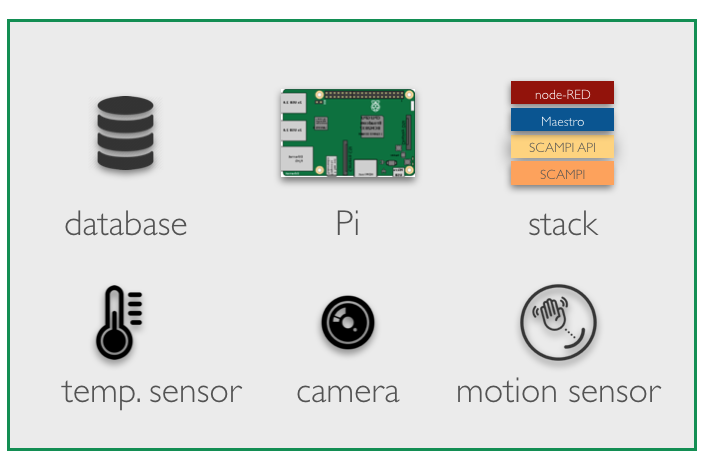
\includegraphics[scale=0.4]{images/node.png}
 \caption{A typical node in the system}
 \label{fig:node}
\end{figure}

\subsubsection{High Performance  Units }

CPUs in the proposed system nodes in \ref{subsub:node}. An example of a high processing unit is  a Graphics Processing unit \textit{GPU}.

\begin{figure}[H]
	\centering
	
\includegraphics[scale=0.7]{images/gpu.png}
		\caption{Figure denoting a Graphics Processing Unit GPU}
	\label{fig:gpu}
\end{figure}

\subsubsection{Network}
\label{subsub:network}
A Network in this design is a set of connected components which are capable of communicating and therefore allowing data sharing between them.
\begin{figure}[H]
	\centering
	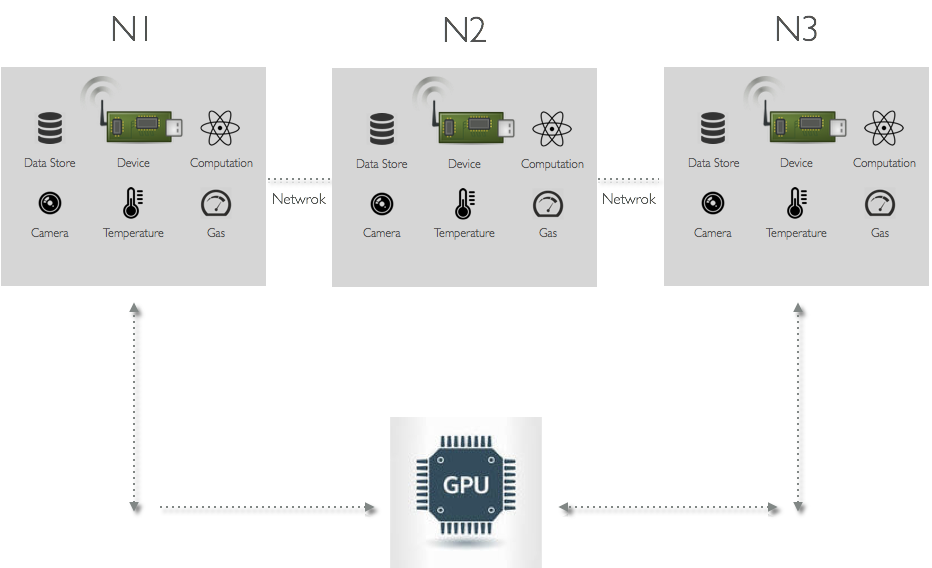
\includegraphics[scale=0.4]{images/network.png}
	\caption{A network consisting of three connected nodes and a GPU}
	\label{fig:network}
\end{figure}
-- TODO: 
Emphasis the difference between persistent and non persistent network links in system design.

\subsubsection{Mobile Device}
A Mobile Device in this context is any device that can connect to the network containing the nodes and is allowed to  carry data from one network to another, hence, allowing a form of data sharing between networks or nodes which are not connected.

\begin{figure}[H]
	\centering
	
\includegraphics[scale=0.3]{images/mobile.png}
	\caption{Figure denoting a Mobile Device}
	\label{fig:mobile}
\end{figure}



\subsection{Connectivity and Data Flow}
A Network described in \ref{subsub:network}, is a simple form of connectivity between components, however, components and specifically nodes are not necessarily connected, sometimes they are just a standalone component that cannot share any information via direct connectivity, also, networks could be disconnected as well, meaning, a network might not be connected to the whole system, thus, is a standalone network. In these cases, a mobile device could help in carrying information and data between these disconnected nodes or networks. 

\begin{figure}[H]
	\centering
	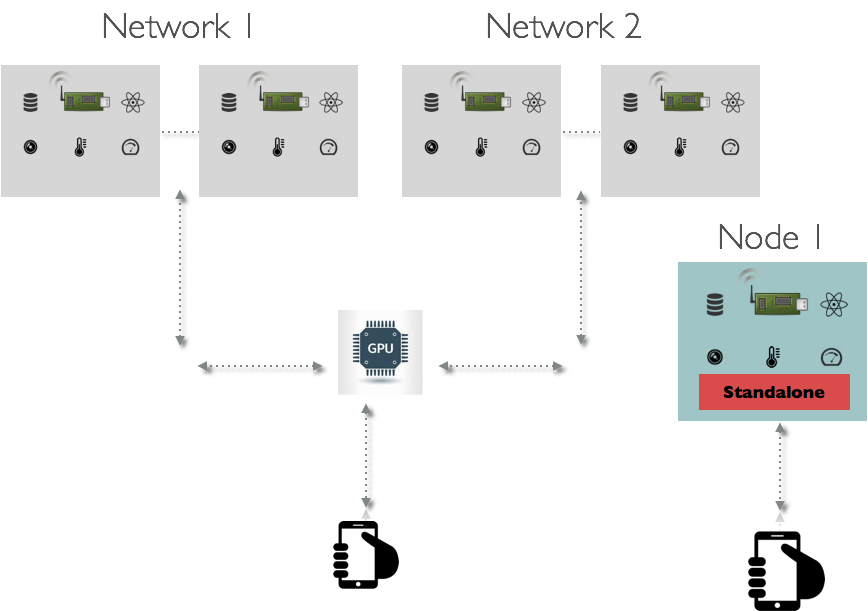
\includegraphics[scale=0.5]{images/system.png}
	\label{fig:system}
	\caption{Two networks connected with a GPU and one standalone network}
\end{figure}









\section{Summary}




% !TeX root = ../main.tex
% Add the above to each chapter to make compiling the PDF easier in some editors.

 \chapter{Approach}\label{chapter:Approach}
 In this chapter we explain the use cases and requirements to design a context-aware pervasive software framework. Then, we illustrate the  proposed architecture and design following from the concepts introduced in the background chapter and taking into account the challenges and possible solutions shown in the foundation chapter. To recap,  our aim is to design a context-aware pervasive software framework to manage and distribute computations while considering resources, dependencies and networking even with an end-to-end path.

\section{Use Cases}
This section provides real life scenarios targeted by framework. Requirements are then elicited from the use cases and then the framework implementation and design is evaluated against these requirements. Note that; the idea of framework is not just to implement these use cases, but to provide the ability to distribute, compose and execute various use cases for context-aware pervasive computing. The use cases are mainly targeted to help human beings, increasing their life quality and preserve the environment. 

\subsection{Smart Cities}
One of the most researched areas in the field of IoT is making our cities more advanced, connected and helpful to human beings and the environment. Researchers and professionals have had many ideas to make use of the context-aware sensor networks that can communicate and act independently whenever the situation needs intervention. We take some examples of the smart cities application and show how they can be implemented using our software framework.

\subsubsection{Smart lighting}

Smart lighting is a use case for automatic control of outdoor lamp posts hence optimizing costs for the governments and enterprises in addition to helping the environment by saving energy \cite{6740844}. The outdoor lighting can be automatically started or closed according to certain circumstances. For example, by lighting up when motion is detected   around it and turning off when there is no further motion, or by detecting natural light  and weather circumstances. Moreover, the lamp posts can be monitored in order to see when a lamp needs replacement.  Further, lamp posts can detect what is the best lighting percentage in a certain situation according to a machine learning algorithm based on the history of decisions taken and feedback provided by users.  In order to implement this use case in our proposed software framework, we must be able to distribute a computational flow to all lamp posts using a messaging system.  Also, the flow should be able to access sensors and be capable of adjusting the light according to the input gathered from several sources including motion, light and humidity sensors.  The decisions taken  should  be   stored into a database so that the flow can access  previous decisions in order to asses the current situation. In addition, a flow with an endpoint that  allows users send feedback on the lighting system can be locally composed to enhance the learning algorithm. Having sent the computational flow to all the lamp posts, the framework should ensure that it does not get deployed on lamp posts without the  required resources, sensors and actuators. 

\subsubsection{Smart Parking}

Automatically detecting empty parking spots in crowded streets is the main idea behind smart parking \cite{4543911}. Since the number of vehicles on the streets are in tremendous increase nowadays, the urge for finding a parking spot in city centers and crowded places has also increased. Having a smart parking mechanism helps in wasting less time, decreasing energy consumption and maintaining a clean environment by reducing emissions.  Different information sources can be used to  detect empty parking spots, for instance, image and video footage of street cameras, crowd sourcing of information and APIs for parking services. Implementing this use case has almost similar requirements to smart lighting, however, it adds having  a camera integrated with smart devices which might produce the need for streaming the footage in real-time to other devices.

%\subsubsection{Crowded Subway Cars detection}
%Using the subway as a mean of transportation in the rush hour can be troublesome, most subway cars are crowded in that time. However, in some of the cases, people in the cars are not normally distributed meaning some cars may be less or more crowded than the others. In this sense, people %thought of using cameras, sensors and actuators to signal people for the less crowded cars. 



\subsection{Mining Applications}

In mining fields it is necessary to always monitor gas and temperature levels in order to prevent miners suffocation \cite{doi:10.1155/2013/159273}. At the same time, it is very hard to maintain a connection between sensors in the inside and  monitoring systems outside \cite{ginzboorg2010dtn}. Therefore, the devices incorporated with sensors inside the fields are expected to be pervasive and warn miners from unexpected increase of gas levels on their own. In addition to delivering the data to the outside world, the system must be able to gather data about the situation inside. This requires miners to act as middlemen who store delay-tolerant data into their mobile devices and carry it forward to the outside world. Of course the miners cannot do this process manually, therefore, there should be a messaging system on their mobile devices that carry the data and handle the synchronization with other device. Also, carrying the data in and out is not the only issue, importing and visualizing  data in the monitoring system should be also done automatically.\\

\noindent The mining use case is a delay-tolerant application because there is a big chance there are no wiring going in and out of the mine where the tunnels are constructed thus a delay-tolerant messaging system should be used. But also, it is an information-centric  application because data should be globally composed by sending  data from  devices in the mine to be imported in  the monitoring system. Having smart devices installed in the mine means its very hard to target them as endpoints without a valid connection, even if there was one, knowing the host names of these devices will still be an issue. Same applies to the monitoring system outside,  data cannot be sent to a specific host name, rathe sent to whoever is interested in  these data.

\subsection{Privacy and Security}
The surveillance systems used at the moment upload  tapes, images and footage of people using public transportation to the cloud and then apply facial recognition algorithms in order to  detect faces of wanted criminals. Despite this being of  significant importance to the national security, this puts everyones privacy in deep water. Therefore, we thought of replacing this model by a pervasive one, where  the facial detection algorithm and faces of  wanted criminals are pushed to the smart devices in public transportation means and whenever a match is found the national security is notified. This helps greatly in increasing privacy, decreasing  latency between the footage and detection in addition to minimizing network bandwidth since the streaming footage  will not be uploaded to the cloud unless there is a match. Similar approaches were introduced in \cite{4653063} and \cite{winkler2010trustcam} where the footage is analyzed on spot to protect privacy. Nevertheless, this is not trivial, facial recognition algorithms are complex and depends on other libraries and  detection models. Therefore, the computation which includes the recognition algorithm  must be able to carry dependencies otherwise the computation will not run. Moreover, the national security should be able to update the list of criminal faces thus messages sent to the smart devices should allow also attachments and dependencies as well. 


\section{Requirements} \label{sec:requirements}

What follows is an enlisting of  the requirements extracted from the real life use cases mentioned in the previous section. We then  evaluate the design and implementation of the framework according to the derived requirements which are  classified  in the following points:
%The framework should
\begin{enumerate}
\item \textit{Service discovery}: since we do not know the host names of the smart devices nor their addresses, the framework should have service discovery mechanism encapsulated in the messaging system as explained in Section \ref{subsec:pub-sub}  to discover peers and  allow any interaction between smart devices.
		
\item \textit{Send and deploy computations}: whatever the use case may be, one of the main requirements of this work, is to be able to send computations to smart devices. This includes sending to one, a set or all smart devices connected together in a network. However, to deploy a computations, the receiving side must have the required hardware resources, sensors and actuators to be qualified for deploying the computation.
 
 \item \textit{Computation dependencies}: complex computations which cannot be executed using the basic operating system and common libraries installed on the smart devices, should carry their  own custom dependencies in order to guarantee a successful run on the receiving smart devices. 


\item \textit{Disconnected devices}: since the framework is also designed to be used in challenged networks, isolated devices in separate networks should also send and receive data or computations using the delay-tolerant architecture.


\item \textit{Communication}: smart devices should be able to communicate, send and receive data in an information-centric and a publish-subscribe manner.

\item \textit{Global identifier}: each smart device must have its own unique global identifier which can be used to send data and computations to this device only.

\item \textit{Composability}: the framework should allow composing multiple computations either locally through a database or globally by allowing data exchange via the publish-subscribe messaging system.

\item \textit{Pervasiveness}: each computation should be able to act on its own, trigger actuators, persist data and access resources such as cameras and sensors if required by the use case.
\end{enumerate}

\section{Framework Architecture}\label{sec:design}
This section explains the software framework architecture designed for pervasive environments and challenged networks to distribute and manage computations with their respective resources and dependencies.  The main idea behind this design is to harness the features of node-RED to create, deploy and share computations of any kind. In addition to having SCAMPI as an information-centric, publish-subscribe and delay tolerant messaging system that gives the framework the ability to deliver messages even without an end-to-end path. However, node-RED and SCAMPI are two different environments that cannot manage computations, resources and dependencies on their own. They need a middleware to orchestrate the communication between them.\\


\noindent In general the architecture stack on each node should look like Figure \ref{fig:stack}. With SCAMPI at the stack bottom relying only on the JVM. Then on top of SCAMPI is its Java API to communicate with the TCP API of SCAMPI. Afterwards, comes the middleware which acts mediator in between node-RED and SCAMPI. Finally, at the very top exits node-RED to run computations and interact with the user if needed. However, if SCAMPI is used on an android device, there might be no need to run neither the middelware nor node-RED since the device will be  used to transport data from one node to another having no end-to-end path. Below we explain how each component of the system works.
\begin{figure}[H]
	\centering
	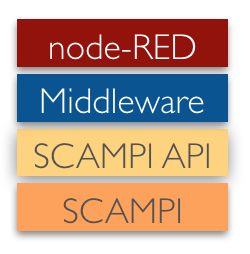
\includegraphics[scale=0.8]{images/stack.png}
	\caption{The framework architecture stack.  }
	\label{fig:stack}
\end{figure}



\subsection{SCAMPI}
As mentioned before SCAMPI is an information-centric, publish-subscribe and delay-tolerant messaging system. In this framework we use SCAMPI to send or receive messages that include computations and data. SCAMPI is also broker-less meaning we do not have to set up a server as broker which is one of the main reasons we chose SCAMPI, in order to be dynamic as possible. The other main reason is to reach nodes which do not have direct connectivity to the publishing node or do not have end-to-end path. \\

\noindent Being a delay-tolerant networking architecture, SCAMPI can use its store-carry-forward routing to deliver messages in challenged environments. In figure \ref{fig:scampi-design}, we show how SCAMPI uses mobile devices to connect nodes that do not have a route or  direct connection and want to exchange messages. In the figure, there are three Raspberry Pi devices running our proposed stack. The first two  have network connection therefore it is rather easy to exchange messages between themselves. However, the third one is isolated, nevertheless it can be connected to a Wi-Fi network or run as an access point. In this case, an android device passing  between network \textit{N1} and \textit{N2} can carry the message bundles from one network and forward it to the other by connecting to both networks alternatingly.  Thus, reaching out to challenged environments that cannot be reached using wired or wireless connections.

\begin{figure}[H]
	\centering
	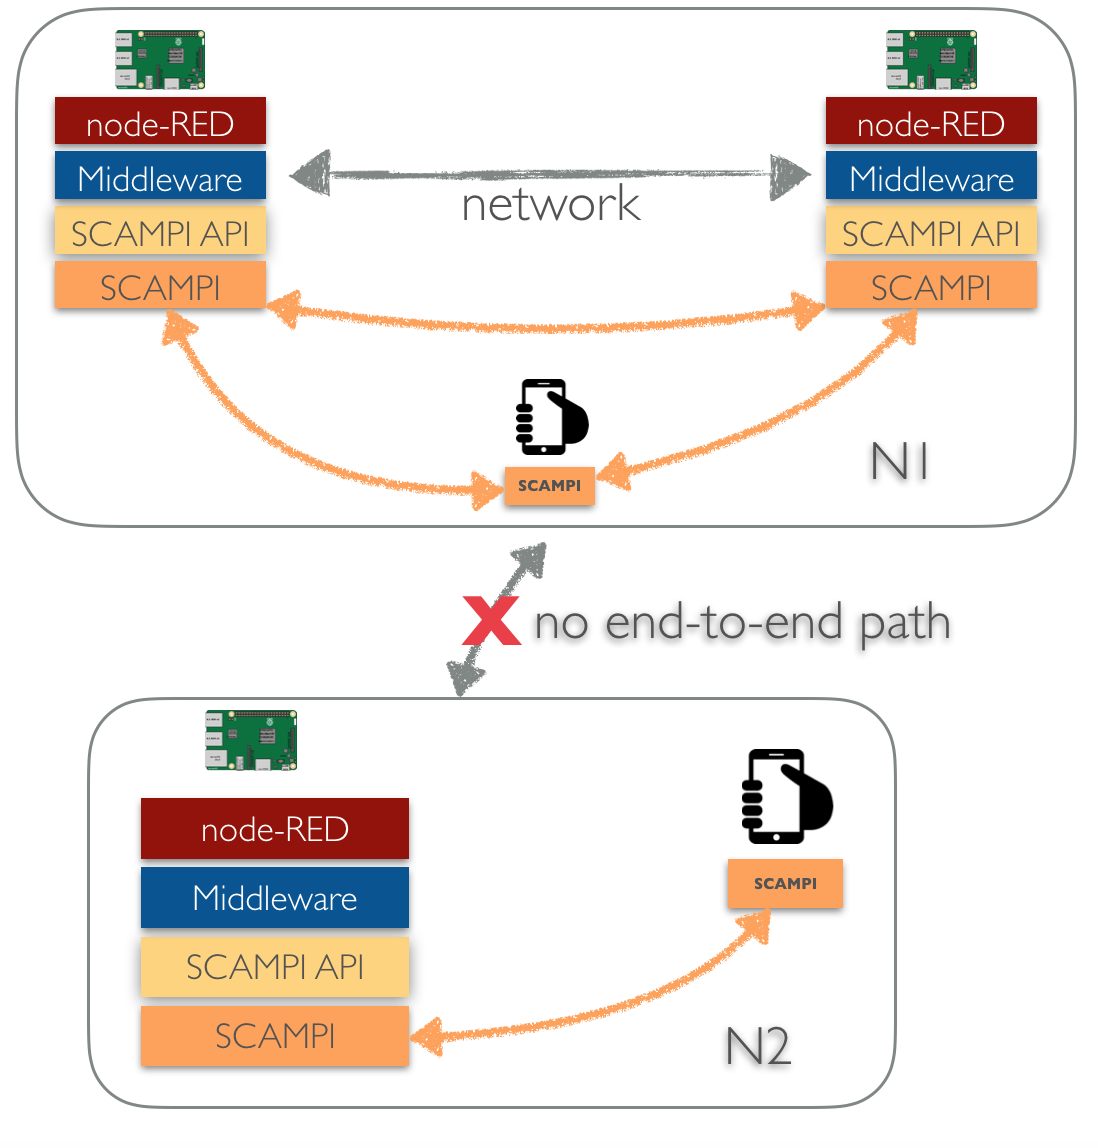
\includegraphics[scale=0.4]{images/scampi.png}
	\caption{SCAMPI synchronization even without an end-to-end path. }
	\label{fig:scampi-design}
\end{figure}

\noindent Being information-centric, data-centric with publish-subscribe pattern and having peer discovery helps us in achieving our dynamic framework without knowing any host names. It  also supports adding and removing nodes at will without any additional configuration. We can also use the general identifiers of the nodes as topics in order to target each of them independently. As stated, SCAMPI does not have any dependencies other than the JVM so we just run it on each node and we are  good to go. \\


\noindent The SCAMPI Java API acts as a client to the server allowing us to publish or subscribe for any topic from the Java environment. Therefore, we are able to extend this API and create a running Java application that uses the TCP API for SCAMPI underneath. The API also allows the client to override the functions for SCAMPI status changes  for instance if it is disconnected, stopped or most importantly when a new message is received. Furthermore, there is a model called \textit{SCAMPIMessage} used to create messages. The model assists in assigning attributes to the message whether strings, integers or even binaries. Also, you can assign meta-data and lifetime to the message.


\subsection{Node-RED}

Node-RED is a tool used for wiring IoT applications, its flows describe the intended computations. It has exporting and importing endpoints for flows via REST which makes it easy to deploy without human interaction.  Flows can be also configured to access certain tables or collections on a running database instance and this configuration can be serialized along with the flow. In this framework whenever a flow wants to send a message to another flow on the same node-RED instance or on other instances, it either uses the REST API that the middleware provides to publish and subscribe to data topics or the same database configuration in both flows to be able to communicate data through the database.. This allows node-RED to send or receive data and allow composability both locally and globally.  Further, node-RED is rich with predefined elements that  can be used to run flows on time intervals, connect to emails, twitter accounts or even access a gpio pin on Raspberry Pi. Node-RED usage is intuitive since it is based on flow-programming, it does not need a developer to create a flow.

\subsection{Middleware}
The middleware is this framework's mediator and the main contribution in this work, it is deployed along with node-RED and SCAMPI on each instance in this architecture. It runs a jar file containing a web application server. It has several duties in orchestrating  SCAMPI messages to node-RED instances.
\begin{itemize}
\item It reads the machine specifications to initialize the machine's resources, sensors and actuators 	.
\item It includes the SCAMPI Java API and has a REST API over it which allows any other script from any other language ("including node-RED") to use the publish subscribe feature of SCAMPI.
\item It analyzes  flows by checking the meta-data  attached to the message thus if the middleware finds out that a flow does not have the necessary hardware requirements, sensors or actuators, it will not deploy the flow. 
\item It is responsible for attaching dependencies of  node-RED flows when one is published, also for putting them into the correct directory when receiving them.
\item It provides a message caching mechanism in order to make sure messages are not handled twice.
\item it provides a mapping between the topics and node-RED flows meaning if one or more flows are interested in the same topic, all of them should get the data.
 \end{itemize}

\subsection{Architecture Usage} \label{subsec:usage}
The following figure \ref{fig:design} explains how the framework works and shows how data flows between the stack components. In this section, we explain the basic usage of the architecture.

\begin{figure}[H]
	\centering
	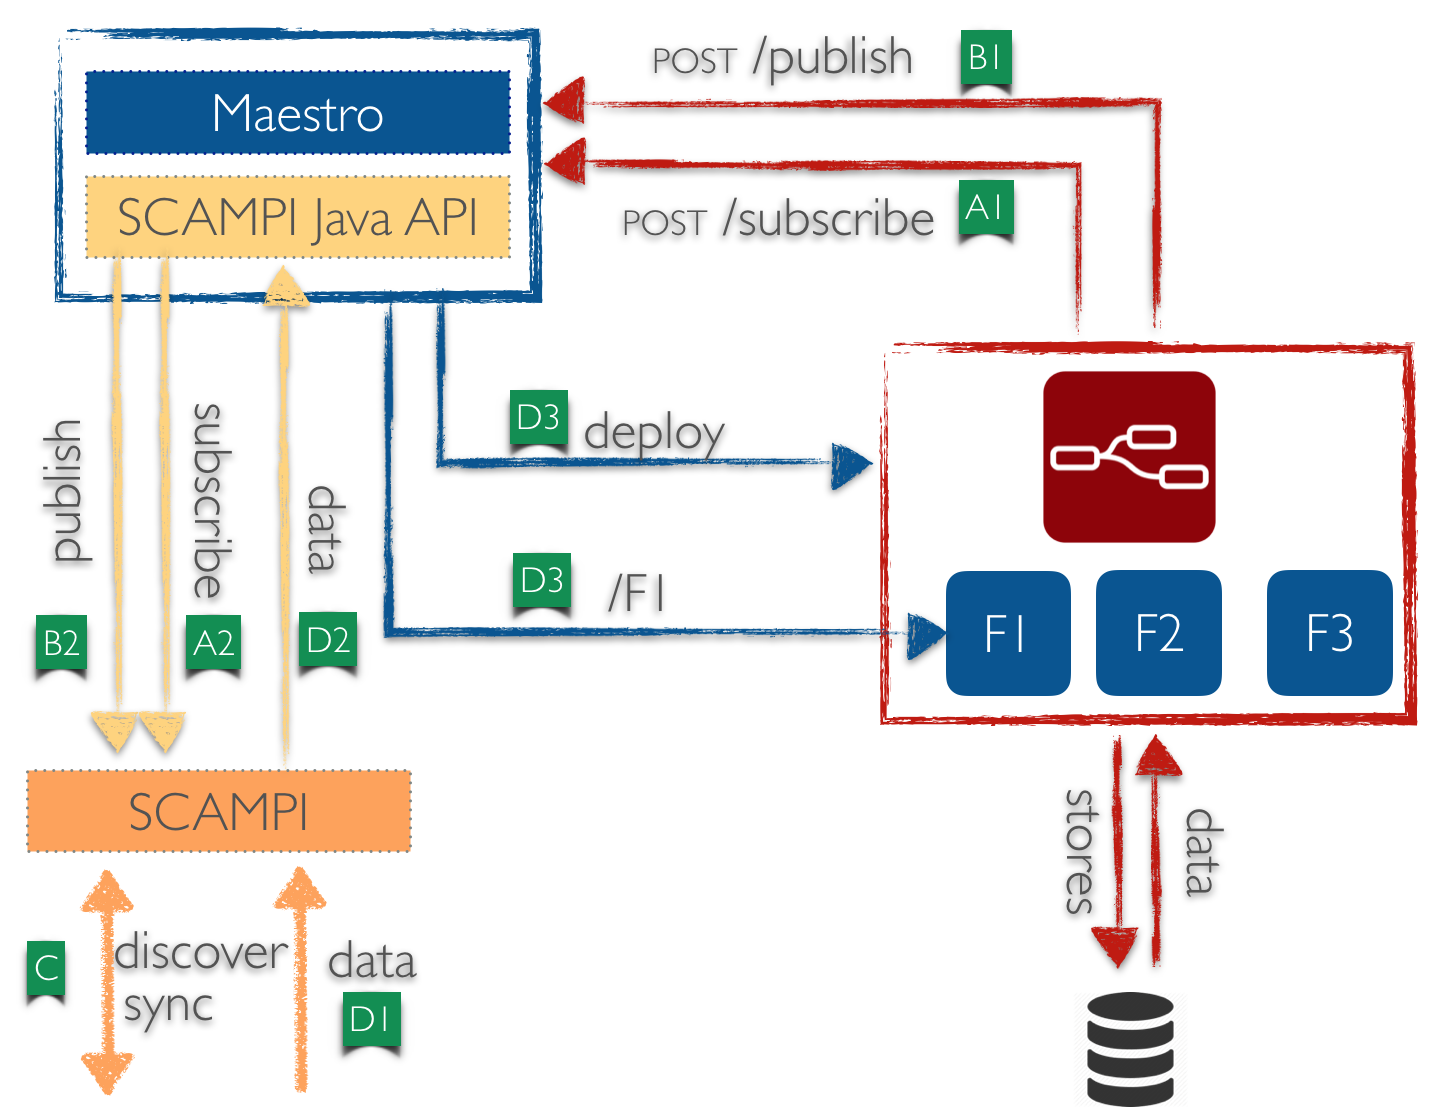
\includegraphics[scale=0.5]{images/design.png}
	\caption{Software framework architecture summary. }
	\label{fig:design}
\end{figure}

\begin{enumerate}[label=(\Alph*)]
 
 \item Flows are developed using node-RED UI, they can include publishing and subscribing REST calls to the middleware. If a flow subscribes to a certain topic, the middelware creates  a topic-endpoint mapping between the topic and an endpoint for this flow specifically. Then send a subscribe request to SCAMPI. If another flow on the same instance wants to subscribe to the same topic, the middleware extends the mapping to include it, hence, once a message is received it gets forwarded to all subscribed flow endpoints. 

 \item When the middleware receives a publish request from node-RED, it attaches the dependencies and an indicator that states if the response should be received by the sending node only. Then the message is forwarded to SCAMPI server.

 \item SCAMPI keeps synchronizing messages and discovering new peers continuously as long as its running. Also, storing some message for the store-carry-forward routing functionality.

 \item When a SCAMPI instance receives data it is forwarded to the middleware, which then checks the meta-data, resources, dependencies and then send the data to the subscribing flows from the topic-endpoint mapping. However, if the message is sent on the computation reserved topic, the middleware will deploy the flow to node-RED.

\end{enumerate}

\section{Summary}

In this chapter we introduced real life use cases for our software framework that was utilized to elicit the requirements used to evaluate the implementation and design of this framework. Afterwards, we described the stack  to implement this framework starting by SCAMPI the  delay-tolerant information-centric messaging system, going through node-RED the platform used to implement, export and execute custom computations serving different use cases, finally we explained the middleware which orchestrates the communication between SCAMPI and node-RED.
% !TeX root = ../main.tex
% Add the above to each chapter to make compiling the PDF easier in some editors.

\chapter{Implementation}\label{chapter:implementation}
Building on the framework architecture explained in Chapter \ref{chapter:Approach}, we describe the middleware proof-of-concept (POC) implementation in details to show that the framework architecture is sound. Moreover we describe the flows implementation used to create the use cases in order tp provide the evaluation for the framework. \\

\section{Middleware}

 The middleware is written in Java, it uses \textit{Maven} as a  software project dependency management which handles the middleware build. \textit{Maven} projects contain a Project Object Model (POM) file which describes the dependencies and libraries used by the project. In addition, it has build configuration management that is used to build the project and create a runnable jar file. The middleware can be compiled and packaged to a jar using the following command \verb|mvn clean package|. The project contains dependencies for \textit{Lombok} which is a library that generates getters, setters and constructors during compile time without the need to write them in the Java classes, \textit{Gson} dependency in order to be able to read and write in JSON format, \textit{SCAMPI API} which allows us to publish, subscribe and override  functions from SCAMPI, dependencies to create a web application via \textit{Spring Boot}. \\
 
 \noindent The project is divided into several packages, we describe them in alphabetical order.
 \begin{itemize}
 
  \item First, the package \verb|com.middleware.api| which contains two classes, \verb|SCAMPApi.java|  and \verb|MiddlewareApi.java|. The class \verb|SCAMPIApi.java| has a field of type \verb|APP_LIB| from SCAMPI Java API which contains the core methods of SCAMPI server to connect, add status listeners, publish and subscribe to messages.  As shown in \ref{fig:cd-api}, \verb|SCAMPIApi| implements two classes via the \verb|APP_LIB| for the SCAMPI server which includes functions like \verb|OnConnected()|, \verb|OnDisconnected()|, \verb|OnConnectFailed()| and \verb|OnStopped()|. It also implements \verb|messageReceived()| which handles the messages once they are received from SCAMPI. Further, It contains a cache for messages and a field indicating the machine specification.
 
The class \verb|MiddlewareApi.java| contains REST API for the middleware web application that runs on port \verb|8080|. It has two requests \verb|POST /publish| and \verb|POST /subscribe|  that connect to  \verb|APPL_LIB| in order to submit publish and subscribe requests to SCAMPI server. The class \verb|MiddlewareAPI.java| has a field for the \verb|topicMapping| which is the topic-endpoint mapping we explained in \ref{subsec:usage}. Last but no least, it has a main method which in Java is used to run a class. In this case, it is used to run the built  jar file from \textit{Maven} which means once the jar file runs via the command \verb|java -jar interface-1.0-SNAPSHOT.jar|, the main method is only thing that runs and therein it starts a web application via \textit{Spring Boot}.
 \begin{figure}[H]
 	\centering
 	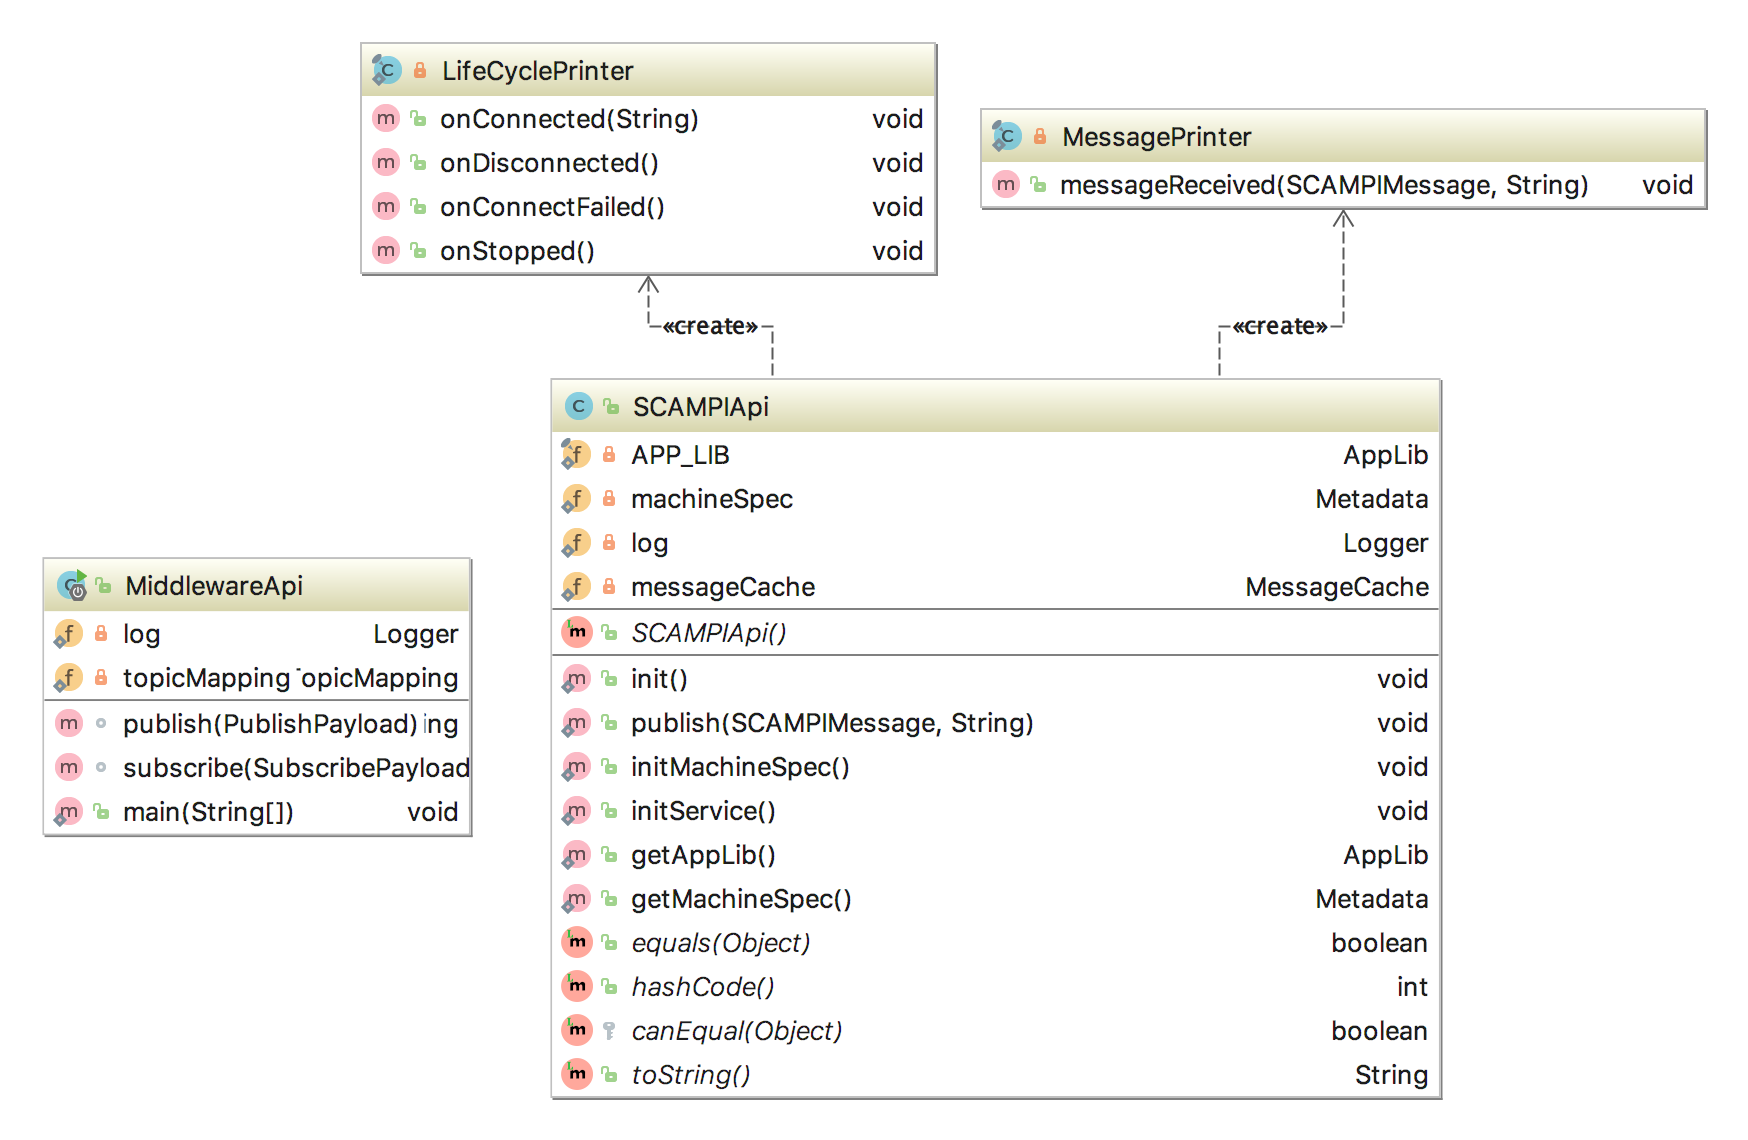
\includegraphics[scale=0.2]{images/cd-api.png}
 	\caption{Class diagram for the api package. }
 	\label{fig:cd-api}
 \end{figure}
 
\item The second package is called \verb|com.middleware.constants| and has one class \verb|Constants.java| which contains all the constant fields used in the middelware across all other classes. This includes string keys for SCAMPI messages, some Linux commands,  URL for the local node-RED instance, path for user home directory on the hosting machine and path for the JSON file that includes the machine specification. Furthermore, it contains the topic reserved for computations named \textit{Main} \\
 
 
 \item The third package is the most important one \verb|com.middleware.domain| which contains most of the services that is handled by the middleware. There are two singleton classes namely \verb|ToppicMapping.java| and \verb|MessageCache.java| that means there exist only one instance across the whole web application no matter how long it runs and no other class can create a new instance of these types. Thats because both are types of caches which should be consistent and global to any class which would need these caches. 
 
 The classes \verb|CommandRunner.java| and \verb|RESTHandler.java| are helpers. The first is used to run commands on the machine and  has two methods \verb|run(String)| and \verb|getFreeRam()| which is equivalent to calling \verb|run("free -m" )|. The second class is used as a REST client for sending requests to node-RED which are used to deploy computations and  send data to endpoints.
 
  Next are the classes \verb|MessageHandler.java| and \verb|Publisher.java| which contain the services for handling incoming messages from SCAMPI and publishing new message respectively. The \verb|MessageHandler.java| is called from  \verb|SCAMPIApi.java| method \verb|messageRecieved()| and differentiates between two types of the messages; computation ones which are received on the topic \textit{Main} and handles them with the method \verb|handleMainTopic(SCAMPIMessage)| which takes care of the resources, machine specifications, puts dependencies on node-RED local directory then the \verb|RESTHandler.java| class is used to deploy the computation to node-RED, and data messages which are received on other topics and handles them with the method \verb|handleSpecialTopic(ScampiMessage)|, it sends the data to any subscribed endpoint in the \verb|toppicMapping| cache using also the \verb|RESTHandler.java|.
 
 The \verb|Pubisher| is responsible for submitting publish requests to the \verb|APP_LIB|. It is called from the \verb|MiddlewareApi.java|.  It creates a unique identifier for each new message, and adds the publisher global identifier to the \textit{SCAMPIMessage} as well. It has the same topic differentiation as \verb|MessageHandler.java|.
 On the one hand, if the publish topic is \textit{Main}, it collects the dependencies and attach it to the \textit{SCAMPIMessage} before it sends the message to SCMAPI server. On the other hand, if it is a data topic it checks the attachments and adjusts the response endpoint  to whether it should be sent back to this node only, if this is the case, it creates a mapping between the global identifier of the node and the endpoint that sent the publish request then send it to SCAMPI server. \\
 
 \begin{figure}[H]
 	\centering
 	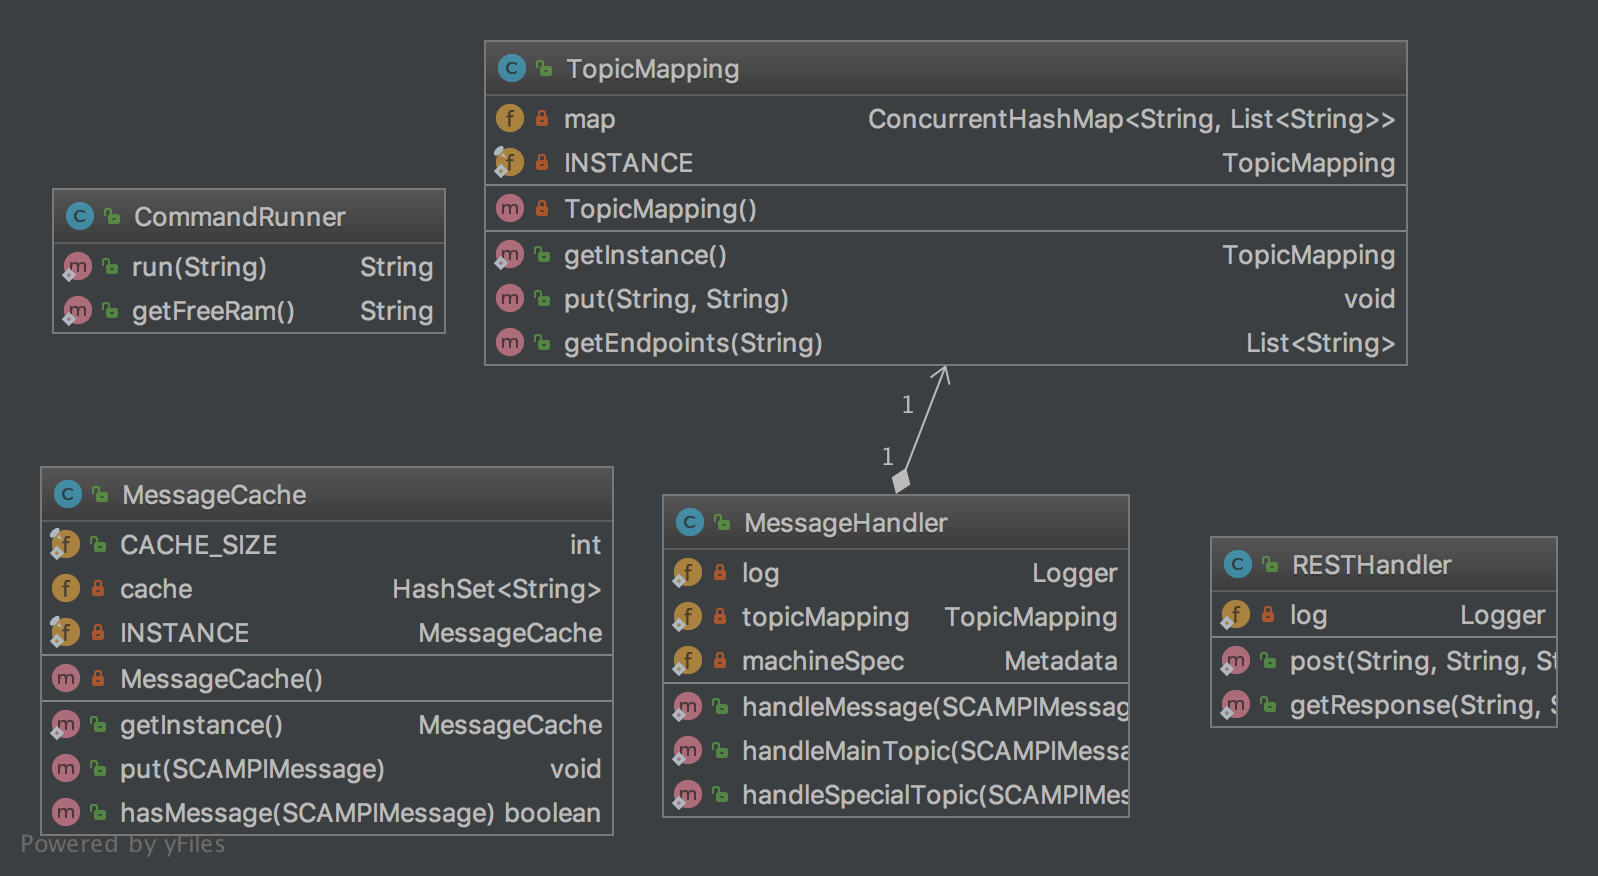
\includegraphics[scale=0.25]{images/cd-domain.png}
 	\caption{Class diagram for the domain package. }
 	\label{fig:cd-domain}
 \end{figure}


\item The fourth package \verb|com.middleware.exception| which contains the project's custom exceptions. Currently it only has a \verb|RESTFailedException.java| class which handles node-RED deployments and data requests failures.

\item The fifth and last package is \verb|com.middleware.model|, it holds the models which are classes used to hold data and encapsulate them. Note that the Java classes do not contain any getters and setters or constructors. However, using \textit{Lombok} library they are generated in compile time and they can be picked up by the Integrated Development Environment (IDE) as shown in \ref{fig:cd-models}. 

 \begin{figure}[H]
	\centering
	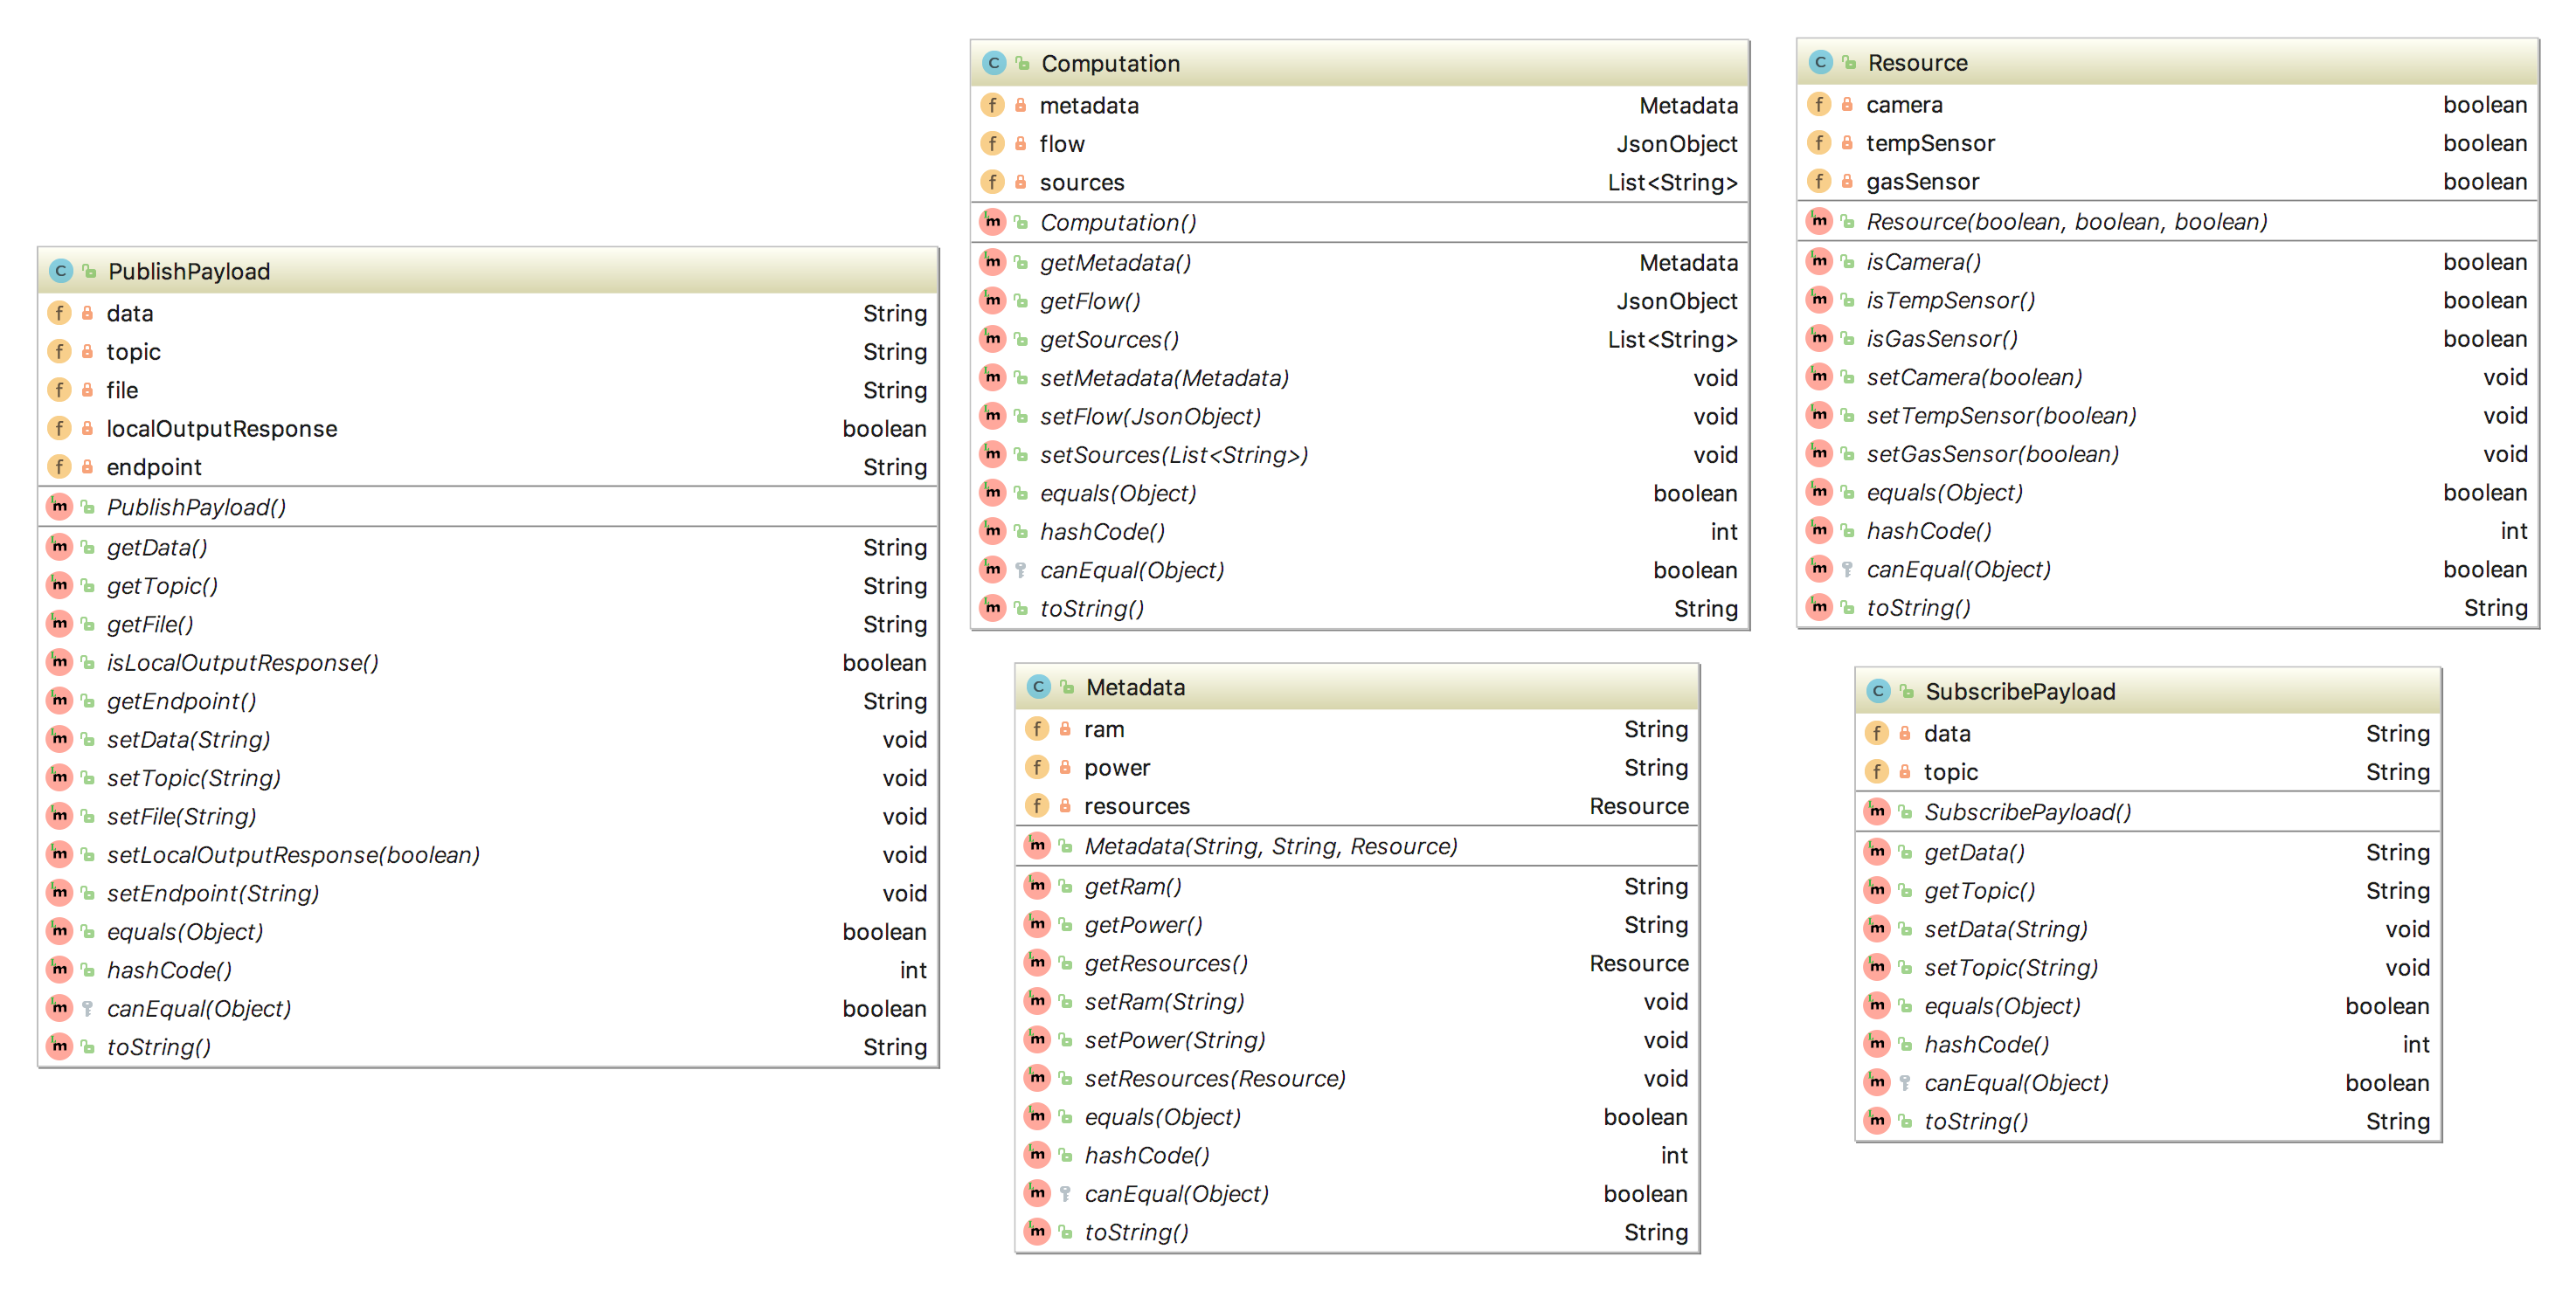
\includegraphics[scale=0.13]{images/cd-models.png}
	\caption{Class diagram for the model package. }
	\label{fig:cd-models}
\end{figure}

\end{itemize}


\section{Flows}
This section explains all the flows developed in this thesis. It shows how the flows can be implemented to achieve different use cases. It also shows how we use node-RED flows in order to send computations.
\subsection{Send Computations}
In order to deliver flows which expresses computations for all nodes or selected ones according to available resources,  sensors, actuators and also attach dependencies, we developed a node-RED flow shown in figure \ref{fig:flow-publish-computation}. The flow responds to the endpoint \verb|GET localhost:1880/publish| and returns the HTML page in figure \ref{fig:html-publish}. Afterwards, the user can adjust the computation power needed by the flow, necessary free Random Access Memory(RAM), sensors and actuators. Then he/she must also write the flow identifier and attach dependencies, and eventually click on the button \textit{push}, which calls another endpoint on the same flow \verb|localhost:1880/push|, it receives the data, fetches the flow details and publish it to the middleware which handles the rest.
 \begin{figure}[H]
	\centering
	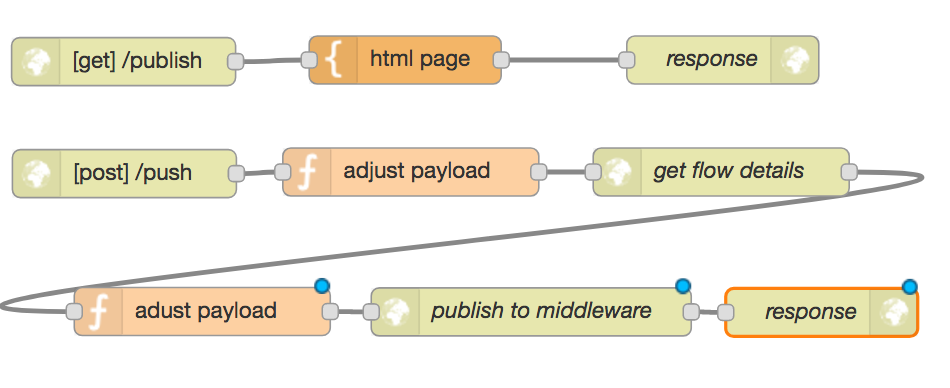
\includegraphics[scale=0.6]{images/flow-publish-computation.png}
	\caption{A flow that publishes computations to the middleware dn thus to SCAMPI.}
	\label{fig:flow-publish-computation}
%\end{figure}
 %\begin{figure}[H]
	\centering
	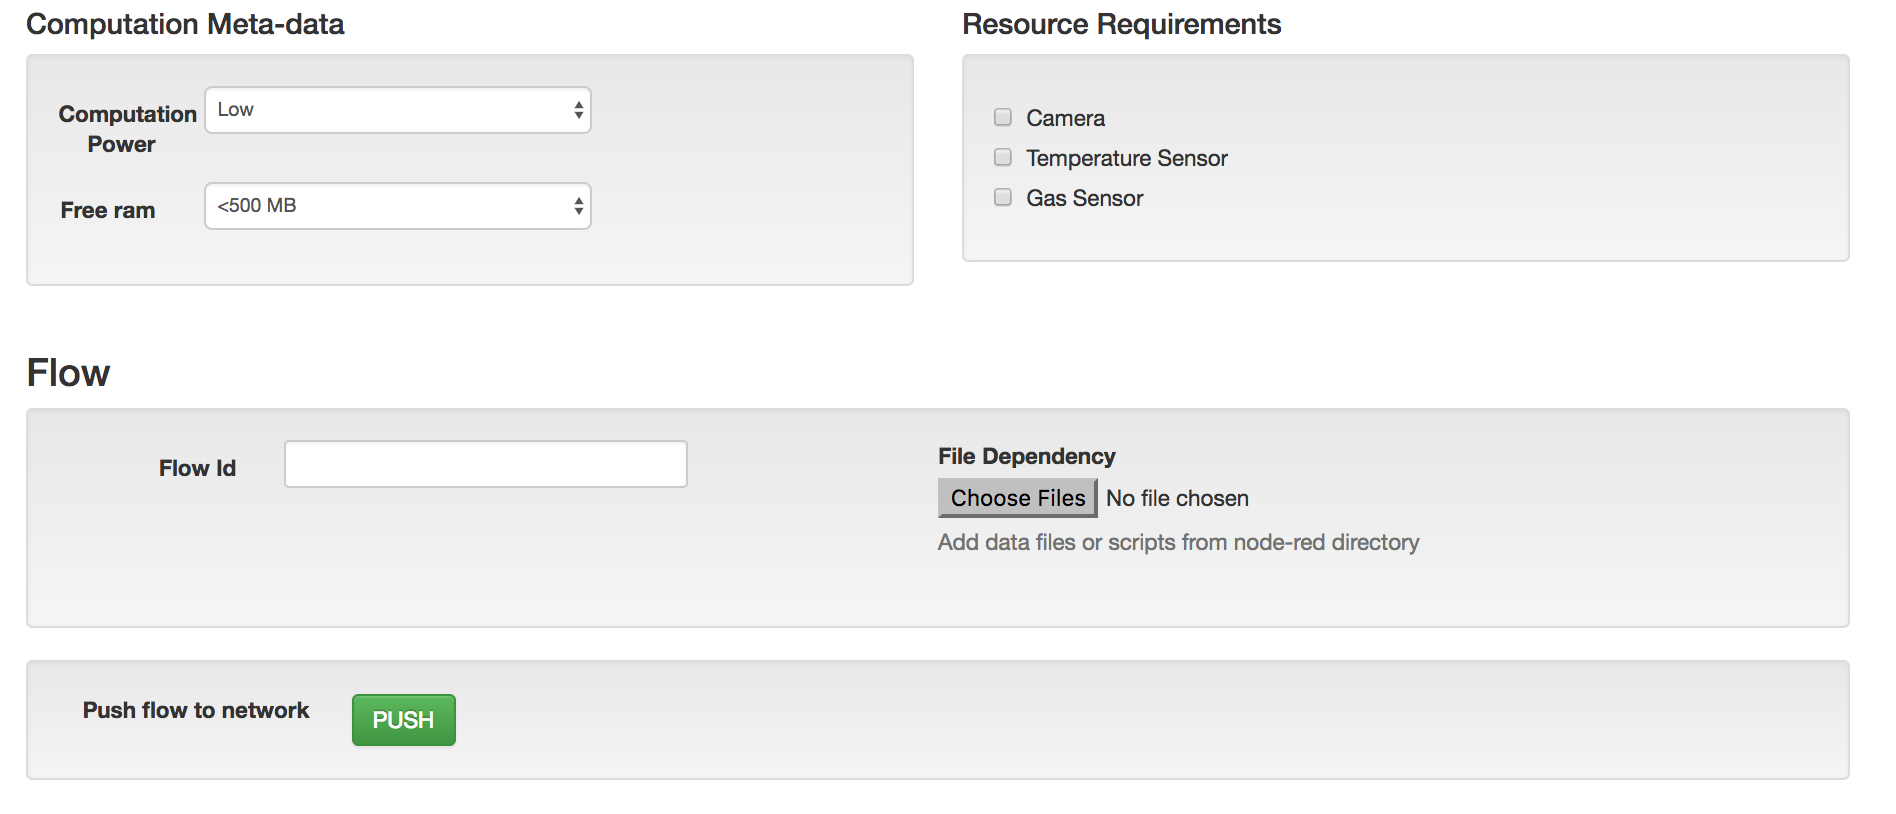
\includegraphics[scale=0.4]{images/html-publish.png}
	\caption{The HTML page used to publish computations conveyed in \textit{html template} element.}
	\label{fig:html-publish}
\end{figure}


\subsection{Temperature Sensor Alert}
This flow was developed to make sure that the software framework works against the basic IoT usage of sensors, actuators and time-series databases. As presented in figure \ref{fig:flow-temp}, the flow runs once it was deployed to any node. Note that it would not have been deployed by the middleware without checking that it has the required resources and dependencies. Once the flow is deployed, it starts a script for sensing temperature  which is sent as a dependency while sending the flow to other nodes. It then checks if the temperature is a valid number, then it gets stored in a database. Further, if the temperature is above 30 degree Celsius it runs a script, which is also sent as a dependency, to light a red led lamp. On top of that, the flow responds to the endpoint \verb|localhost:1880/temp| and returns all the collected temperature data in the last two minutes.
 \begin{figure}[H]
	\centering
	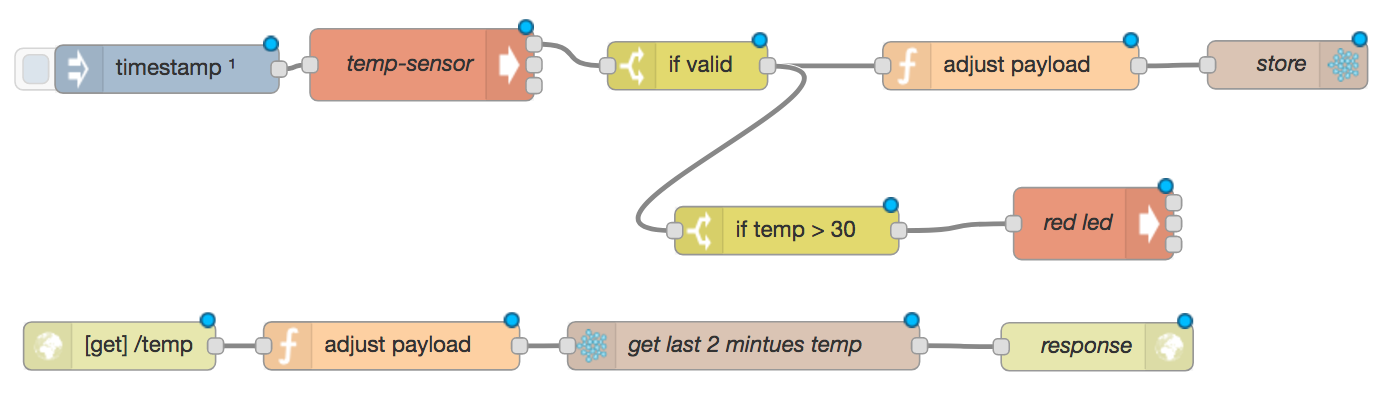
\includegraphics[scale=0.6]{images/flow-temp.png}
	\caption{A flow that reads temperature and stores it, also start a red lamp if temperature is above 30 degree Celsius.}
	\label{fig:flow-temp}
\end{figure}



\subsection{Detect Movement and Store Image Responses} \label{subsec:detect-move}
As part of the implementation evaluation, we developed this flow to take part in a bigger use case. The flow is designed to detect movement through the infrared sensor and then take a picture, which is then published on the topic \textit{NUC} for image recognition. However, in the push payload along with the picture, there is a field stating that the response should come back to this exact node, therefore, the middleware creates a mapping between the device global identifier and the endpoint before publishing. Also, as demonstrated in \ref{fig:flow-motion}, the flow awaits messages on its endpoint and executes a script which starts a red led, it also store the recognized image in a database along with its accompanying data. 

\begin{figure}[H]
	\centering
	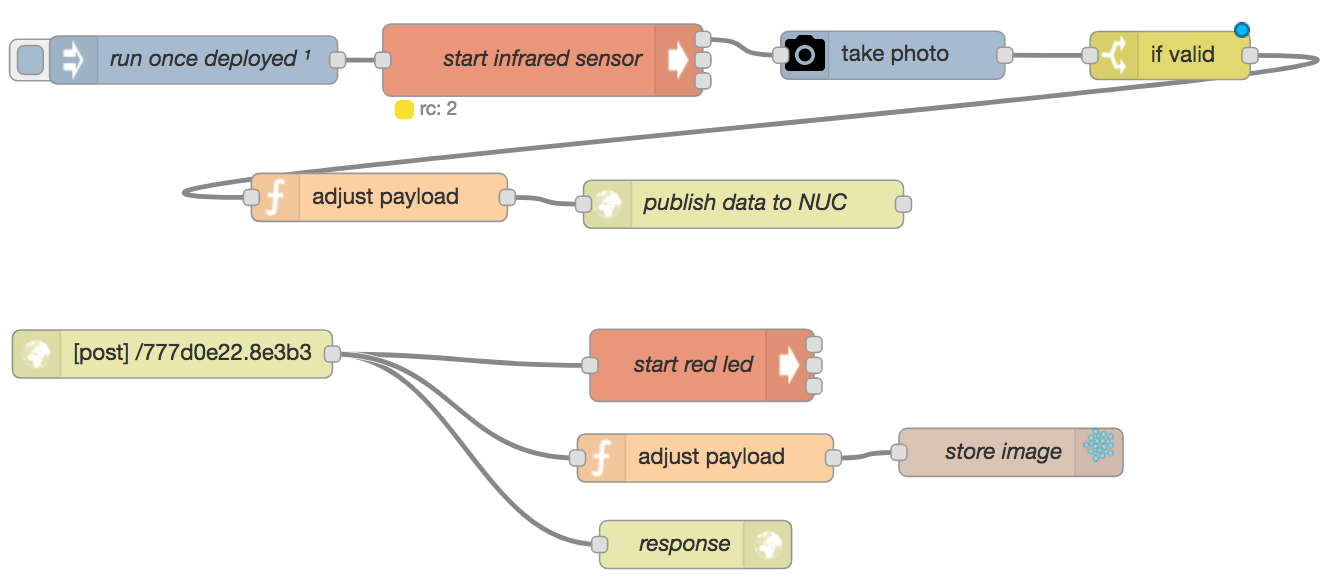
\includegraphics[scale=0.6]{images/flow-motion.png}
	\caption{A flow that detects motion, take an image, publish message and store response.}
	\label{fig:flow-motion}
\end{figure}


\subsection{Show Recognized images}
Since compatibility is an important part to validate in our framework. We created a simple flow to show local composable flows. It simply queries the database for recognized images from the previous flow \ref{subsec:detect-move} when requested on the endpoint \verb|GET localhost:1880/images|. It has an HTML page response showing all the images along with their image recognition confidence percentage data and time-stamp.

\begin{figure}[H]
	\centering
	
\includegraphics[scale=0.6]{images/flow-images.png}
	\caption{A flow that creates an endpoint for stored database images.}
	\label{fig:flow-image}
\end{figure}

\subsection{TensorFlow Water Bottle Recognition} \label{subsec:tensor}
To prove that we can send flows to machines with heavy computation power and lots of free RAM. We developed an image recognition flow using \textit{TensorFlow} which is an open-source software library for machine intelligence. \textit{TensorFlow} needs a 54MB image recognition model that recognizes 1000 object classes, one of them is a water bottle. It also needs the code to run the recognition algorithm which is a Java jar file of 29MB size. Therefore, the flow  needs to carry all the mentioned dependencies. As show figure \ref{fig:flow-tensor}, the flow subscribes to the topic \textit{NUC} once it is deployed. Then, when the middleware that runs on the same machine receives a message on the topic \textit{NUC}, the middleware sends it to the corresponding endpoint  from the topic-endpoint mapping, it also puts the dependencies in node-RED directory. Thereafter, the flow uses the message payload which should be an image, and runs the jar. If it results in a water bottle as a best match, the flow responds to the sender with the result and a confidence percentage.
 \begin{figure}[H]
	\centering
	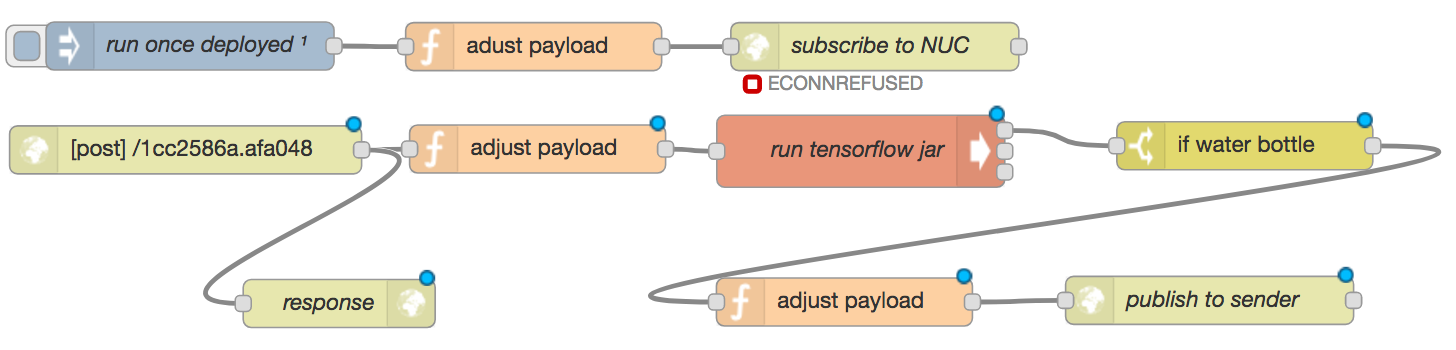
\includegraphics[scale=0.6]{images/flow-tensor.png}
	\caption{A flow that uses tensorflow to recognize a water bottle.}
	\label{fig:flow-tensor}
\end{figure} 

\section{Starting the framework}\label{subsec:starting-framework}

The framework stack is run in the following order; SCAMPI, middleware and then node-red. The script used for starting the stack is as follows:
\begin{verbatim}
#!/bin/bash
java -jar SCAMPI.jar default_settings.txt > scampi-log.txt 2>&1 & disown
sleep 10
java -jar interface-1.0-SNAPSHOT.jar > interface-log.txt 2>&1 & disown
sleep 5
node-red > node-red-log.txt 2>&1 & disown
echo "All Set Up"
\end{verbatim}
There is a sleeping period between each command in order to make sure that the previous one has started. The commands have to be executed in this order, however, if the middleware starts before SCAMPI it will not break and keep waiting for the server to start. But, node-RED must wait for both of them to start, as there are flows that only executes at the time of deployment, therefore the whole stack has to be running at this point. Note also, that there are logs for each process that can be found in the node-RED directory. 
% !TeX root = ../main.tex
% Add the above to each chapter to make compiling the PDF easier in some editors.

\chapter{Evaluation}\label{chapter:Evaluation}

The goal of this chapter is to validate the framework architecture design for context-aware pervasive computing in challenged environments which was described in Chapter \ref{chapter:Approach}. It also evaluates the middleware implementation which was explained in Chapter \ref{chapter:implementation}. Note that, the delays and performances are to be taken with a grain of salt, as the system is designed as a proof-of-concept and not to run in production systems. \\

\noindent In order to evaluate the framework and implementation with all its requirements, we divided the evaluation into several use cases. The devices used for  the use cases has different hardware capabilities. They might also have  sensors and actuators according to each use case. All the devices must be running our stack framework as explained in \ref{subsec:starting-framework} except for android phones which has \textit{Liberouter}, an implementation for SCAMPI on android phones. The devices we used in this evaluation are:
\begin{center}
	\begin{tabular}{ c | c | c| c }
		
		Name & Count & Stack & Performance \\ \hline
		 &  &  &  \\
		Intel NUC &1& 	Our framework &   \specialcell[c]{CPU:Intel Core i5-6260U Processor\\ (4M Cache, up to 2.90 GHz)\\RAM: 16GB }\\ 
		&  &  &  \\
		Raspberry Pi 3 model B & 2 & Our framework &  \specialcell[c]{ CPU: 1.2GHz\\RAM: 1GB}  \\ 
		&  &  &  \\
		HTC one M9 & 1 & Liberouter &   \specialcell[c]{CPU: Octa-core \\4 x 2.0GHz + 4 x 1.5GHz\\ RAM: 3GB} \\ \hline
	\end{tabular}
\end{center}




\section{Recognizing Water Bottles }
 \begin{figure}[H]
	\centering
	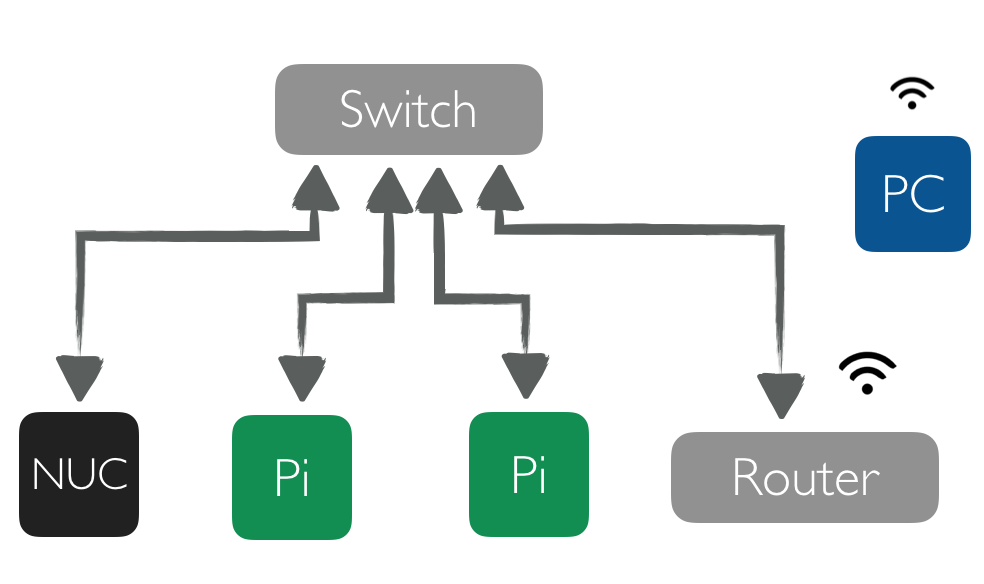
\includegraphics[scale=0.6]{images/tb-tensor.png}
	\caption{Testbed setup for recognizing water bottles.}
	\label{fig:tb-tensor}
\end{figure} 

\section{Challenged Networks}
\begin{figure}[H]
	\centering
	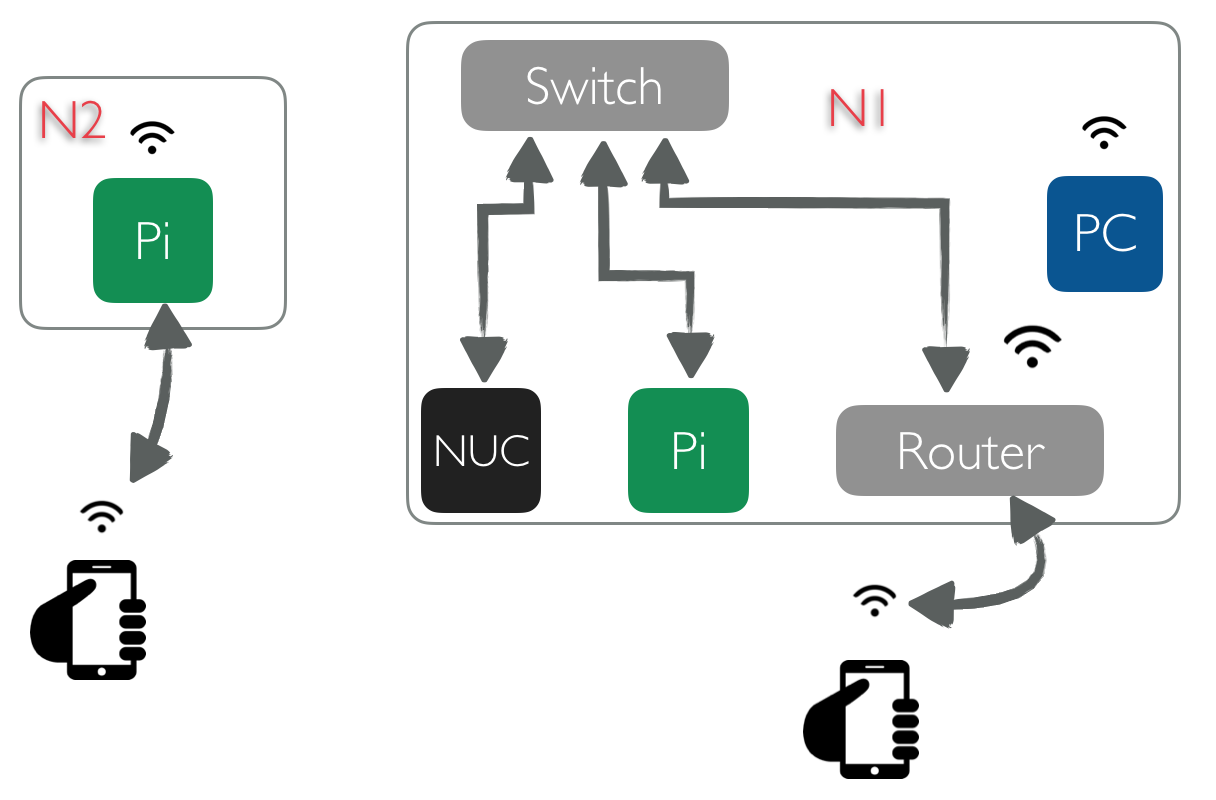
\includegraphics[scale=0.6]{images/tb-dtn.png}
	\caption{Testbed setup for challenged and delay tolerant networks.}
	\label{fig:tb-dtn}
\end{figure} 

\section{Basic IoT Usage}
% !TeX root = ../main.tex
% Add the above to each chapter to make compiling the PDF easier in some editors.

\chapter{Conclusion}\label{chapter:conclusion}

This chapter concludes the work of this thesis, we first give a summary about the proposed software framework,  thesis flow and  main contribution of this work. Second, we demonstrate the results and  outcome of this thesis. Finally, we discuss the future work and enhancements for  this work. 

\section{Summary}
To sum up, we designed and presented a delay-tolerant and information-centric framework architecture for pervasive computing  that distributes, composes and executes flows which are representations of computations describing pervasive use cases. The framework uses  service discovery, allows sending and receiving of flows while accounting for their dependencies, required hardware resources, sensors and actuators even without an end-to-end path between senders and receivers. Moreover, it provides the execution environment for the flows and a user interface for publishing and designing flows. Further, the framework allows devices to communicate with each other and exchange data in a publish-subscribe manner which enables them to compose and have inter-relationships in addition to  being able to locally exchange data through databases hosted on the same device. \\

\noindent In this thesis, we first gave an introduction about the problem and our intent to design a pervasive framework for computation distribution, composition and execution even in challenged networks. Therefore in the background chapter, we researched the current accomplishments in the fields of pervasive computing, delay-tolerant and information-centric networking. After harnessing these concepts and architectures we came up with ideas and foundations which led us to design our framework architecture. However, in order to evaluate it, we needed concrete real life use cases for  requirements elicitation so that we can evaluate our framework against these requirements which were discussed in the approach chapter. We also explained middleware implementation and used the extracted requirements to devise experimental use cases to evaluate our framework.\\

\noindent The main contribution of this work is both the framework design and the implementation of Maestro which acts as a middleman between the messaging system and the execution environment. It handles the flows necessities by attaching the dependencies, checks the flow meta-data in order to make sure the device meets desired requirements and has the required resources. Once the flow passes all checks, it deploys the flow to the execution environment.


\section{Results}
The evaluation results of our  proof-of-concept implementation and architecture design showed the feasibility of our framework. The use case experiments that we ran satisfied the  requirements which were devised from  real life use cases. We have proved the viability of distributing and executing flows with dependencies to smart devices with different resources and gadgets. Further, we presented that devices can exchange messages and compose different flows locally and globally. Beyond that, we confirmed that messages are delivered to challenged networks that does not have an end-to-end path. Finally, we provided the mean and standard deviation of the delays taken between sending and deploying messages to execution. 



\section{Future Work}
The framework can be extended and enhanced on several aspects:
\begin{itemize}
\item \textit{Streaming}: a possible extension to the framework is to allow live feed or footage to be streamed from one device to another, of course this could be done by composing flows in which one device shoots a video and sends the frames to other devices. However, this might experience some delay, it would be more efficient to have a streaming API in the messaging system which can be exposed to both the middleware and execution environment.

\item \textit{Request-Response Mapping}: In the middleware implementation there is no way at the moment to map a published message sent as a request  with another sent as a response. More specifically, in the challenged networks experiment, we could not be sure which requests for image recognition sent from the Raspberry Pi lead to the successful  replies  sent from the NUC back to the Raspberry Pi. This is not the case with recognizing water bottles experiment because we sent one request each run and waited for the response. Unlike the challenged networks experiment, we sent a lot of requests and received less replies. This could possibly be done by forwarding the unique message identifier from the request to the reply thus mapping between them.

\item \textit{Security}: This thesis does  not focus on securing the communication between devices and ensuring that requests and deployments to the execution environment are authenticated. This could be enhanced by providing a layer of security in the messaging and deployment process.

\item \textit{Resources Discovery}: The current middleware implementation reads the resources from a specification file on the smart devices. It would be more dynamic and flexible if the middleware could discover the attached resources dynamically and sensitive to the addition or removal of gadgets. 

\end{itemize}
\appendix{}
\begin{appendices}
\chapter{Use case Evaluation Results}
\section{Basic IoT Usage Flow}
\begin{table}[H]
	\centering
	\begin{tabular}{c|c|c|c|c}\toprule
		&  $ t_{Pi1} - t_{PC}$   & $t_{db} - t_{Pi1}$  & $ t_{Pi2} - t_{PC}$ &  $t_{db2} - t_{Pi2}$ \\ \midrule
		1& 	4.542& 	1.713& 	4.693& 	1.726\\
		2& 	2.438& 	1.706& 	2.533& 	1.716\\
		3& 	2.885& 	1.701& 	2.065& 	1.717\\
		4& 	2.451& 	1.815& 	2.462& 	1.723\\
		5& 	2.333& 	1.713& 	1.536& 	1.685\\
		6& 	2.423& 	1.724& 	1.444& 	1.727\\
		7& 	3.437& 	1.705& 	2.414& 	1.722\\
		8& 	2.453& 	1.711& 	2.35& 	1.72\\
		
	\end{tabular}
	\caption{Delays for the temperature flow.}
	\label{table:temp-results}
\end{table}

\section{Recognizing Water Bottles Experiment Delays }\label{app:tensor}
\subsection{Image Recognition Flow }
\begin{table}[H]
	\centering
\begin{tabular}{ c | c | c| c }	\toprule
\$ &$t_1 - t_0$  & $t_2 - t_0$  & $t_3-t_0$ \\ \midrule
1&	23.245&	28.226&	20.826\\
2&	20.699&	49.666&	19.051\\
3&	22.330&	21.756&	29.425\\
4&	21.387&	22.265&	32.680\\
5&	22.549&	27.662&	22.627\\
6&	24.095&	27.222&	15.922\\
7&	19.597&	25.561&	43.311\\
8&	22.586&	26.898&	28.627\\
\end{tabular}
\caption{Delays for sending image recognition flow for all devices.}
\label{table:tensor-results}
\end{table}

\subsection{Detect Movement and Store Image Responses Flow}
\begin{table}[H]
	\centering
\begin{tabular}{ c | c | c| c }	\toprule
\$ &$t_5 - t_4$  & $t_6 - t_4$  & $t_7-t_4$ \\ \midrule
1&	0.104&	2.386&	2.233\\
2&	0.106&	2.323&	2.348\\
3&	0.090&	2.321&	1.380\\
4&	0.080&	2.340&	1.275\\
5&	0.076& 2.210&	1.441\\
6&	0.081&	2.299&	2.247\\
7& 0.088&	2.329&	2.211\\
8&	0.074&	2.368&	2.450\\
\end{tabular}
\caption{Delays for sending the motion detection flow for all devices.}
\label{table:motion-results}
\end{table}

\subsection{Images and Recognition Results}
\begin{table}[H]
	\centering
\begin{tabular}{ c | c | c| c | c| c }	\toprule
 \$ &$t_9 - t_8$  & $t_{11} - t_{10}$  & $t_{13}-t_{12}$ & $t_{15}-t_{14}$&  $t_{tensor}$ \\ \midrule
1&	0.266&	0.659&	0.276&	0.686&	5.582\\
2&	0.296&	0.674&	0.323&	0.79&	5.640\\
3&	0.186&	0.728&	0.313&	0.676&	5.573\\
4&	0.342&	0.807&	0.222&	0.661&	4.940\\
5&	0.227&	0.752&	0.219&	0.722&	5.603\\
6&	0.262&	0.713&	0.322&	0.742&	5.599\\
7&	0.306&	0.684&	0.212&	0.663&	5.575\\
8&	0.374&	0.582&	0.293&	0.648&	5.581\\
\end{tabular}
\caption{Delays for data sent between the Raspberry Pis and the NUC.}
\label{table:data-results}
\end{table}


\section{Get Recognized Images Experiment Delays}\label{app:images}
\begin{table}[H]
	\centering
\begin{tabular}{ c | c | c| c }	\toprule
	\$ &$t_{17} - t_{16}$  & $t_{18} - t_{16}$  & $t_{19}-t_{16}$ \\ \midrule
1&	0.102&	0.761&	0.838\\
2&	0.163&	0.799&	0.799\\
3&	0.125&	0.927&	0.923\\
4&	0.091&	0.752&	0.868\\
5&	0.070&	0.814&	0.778\\
6&	0.095&	0.824&	0.861\\
7& 0.094&	0.736&	0.835\\
8&	0.098&	0.798&	0.769\\	
\end{tabular}
\caption{Delays for the flow which retrieves the recognized images for all devices.}
\label{table:images-results}
\end{table}


\section{Challenged Networks}
\begin{table}[H]
	\centering
	\begin{tabular}{c|c}\toprule
		& $t$  \\ \midrule
		1&	284.957\\
		2&	216.409\\
		3&	180.415\\
		4&	228.811\\
		5&	228.329\\
		6&	220.11\\
		7&	214.213\\
		8&	111.267\\
		9&	104.166\\
		10&	101.188\\
		11&	179.825\\
		12&	178.946\\
		13&	166.999\\
	
	\end{tabular}
	\caption{ Delays for messages sent from the disconnected Raspberry Pi to the NUC.}
	\label{table:DIS2-results}
\end{table}


\begin{table}[H]
	\centering
	\begin{tabular}{c|c}\toprule
		& $t$  \\ \midrule
		1&	59.531\\
		2&	51.51\\
		3&	51.826\\
		4&	213.212\\
		5&	67.856\\
		6&	67.673\\
		7&	68.188\\
		8&	68.103\\
		9&	64.292\\
		10&	192.479\\
		\end{tabular}
	\caption{Delays for messages sent from the NUC to disconnected Raspberry Pi having successfully recognized water bottles.}
	\label{table:DIS3-trdulyd}
\end{table}

\end{appendices}


\microtypesetup{protrusion=false}

\microtypesetup{protrusion=true}
\printbibliography{}

\end{document}